%\TEX root = ../../thesis_rui_almeida.tex


\section{\acrlong{AP}}%
\label{sec:ap}

Daniel Vallero, in his book "Fundamentals of Air
Pollution"~\cite{Vallero2014} makes a very important observation: Air
Pollution has no universal definition. Its meaning is intertwined with
the context with which it is measured and observed, with the ecosystem
in which it is perceived and even with the pollutant concentration (not
every toxic compound is toxic at every concentration). The \gls{EPA}
defines Air Pollution as the following:

\begin{center}
    \begin{minipage}{0.8\textwidth}

        \noindent \textit{Air Pollution is the presence of contaminants
        or pollutant substances in the air that interfere with human
        health or welfare, or produce other harmful environmental effects.}

    \end{minipage}
\end{center}

He then analyzes this definition through two possible lenses, the one
that comes with the interference produced by air contaminants; and the
one that comes from the harm they may cause. He notes that both points
of view come with a heavy burden of ambiguity, incompatible with a
scientific definition. We can thus observe that preferable to address
the issue through its measurable effects and consequences. These are
well-established and well known, and scientists all around the world
have been publishing extensively about them for some decades now. The
correlation between Air Pollution and an increased mortality in heavily
industrialized areas was first established in Europe, in the
19\textsuperscript{th} century, but the first time it was taken
seriously was during the 1952 killer-smog incidents, in
London~\cite{Platt2007}. At the time, a combination of very cold
weather, an anticyclone and fireplace emissions caused a thick smog to
fall over London, directly causing thousands of deaths and indirectly
many more~\cite{Bell2008,Office2019}. The disastrous consequences of
this incident had a huge impact in the civil society, resulting in a
series of policies and laws, among which the Clean Air Acts of 1956 and
1968, which are broadly considered to be some of the first actions to
decrease pollution in human societies. Much work has been done, and it
has resulted in remarkable progress since the definition of those two
policies. We are in fact in a much better place than we were some years
or decades ago, but pollution is still a part of everyday reality for
the whole of civilization. In the current day and age, both European and
American regulatory and surveillance bodies (the \gls{EEA} and the
\gls{EPA}, respectively) have identified a group of six \emph{criteria
pollutants} that need to be monitored effectively. These gases, whose
effects this section particularly focuses, are presented in
Table~\ref{tab:criteria_pollutants}. In this section, I will present the
most significant aspects of \gls{AP} that are described in the
literature, including health effects, environmental effects and
\acrlong{AP} monitoring.

\begin{table}[htpb]
    \centering
    \caption{Criteria pollutants as defined by the EPA and the
    EEA~\cite{CABI2019}. These are the pollutants whose effect is more
    significant for society itself, given their level of dangerousness and
    how common they are.}
    \label{tab:criteria_pollutants}
    \begin{tabular}{c}
    
    \end{tabular}
\end{table}

\todo[inline]{Criteria Pollutant table}


\subsection{\acrlong{AP} Effects on Human Health}%
\label{sub:ap_effects_on_human_health}

Arguably, there is no medium in which it is more important to consider
\gls{AP} by its effects than in the human body. However, even this has
its caveats. The body's response to any given substance changes with the
dose that is administered to it, something which has been known to us
for centuries:

\begin{flushright}
    \begin{minipage}{0.8\textwidth}
        \noindent
        \textit{
            What is it that is not poison? All things are poison and
            nothing is without poison. It is the dose alone that makes a
            thing not poison.
        }

        \hfill-- Paracelsus
    \end{minipage}
\end{flushright}

This quote, originally in the writings of one of the fathers of modern
medicine, the Swiss Paracelsus, was taken from Patricia Frank's book
called \emph{The Dose Makes The Poison}~\cite{Frank2011} and is one of
the core tenets of toxicology even today. There are, however, some
substances which do not need anything close to a high dose to cause harm
to human health, and in general, atmospheric pollutants fall in that
category. According to the \gls{EEA}, heart disease and stroke are the
most common causes of premature death due to \acrlong{AP}. The same
organization states that the most prominent atmospheric pollutants in
terms of the effects they have on human health are \gls{PM}, \gls{no2}
and \gls{o3}~\cite{EEA2016, EEA2007}. In this thesis, I will focus
mostly on them, not only because of their health importance, but also
because of their spectral nature, which allows us to detect them using
\gls{DOAS}~\cite{Platt2007}. Of course, a complete description of how
\gls{AP} affects the human body is a colossal task which is well beyond
the scope of this thesis.  Therefore, I will focus my attention on the
more prominent symptoms that are results of these chemicals: respiratory
syndromes, cardiovascular diseases, problems during gestation and
finally, neurologic consequences of \gls{AP}.

%%% THIS PARAGRAPH IS WELL WRITTEN, BUT DID NOT FIT THAT WELL
%%%%%%%%%%%%%%%%%%%%%%%%%%%

% It is not the dose alone to make the poison. Rather, one has to consider
% the whole context at which we are directing our discussion. Nitrogen
% compounds in the air cause several respiratory syndromes, but in the
% soil they are essential nutrients~\cite{Vallero2014, Lovett2009}.
% Admittedly this is an extreme comparison, but it serves to introduce the
% reader to the concept of dependence between the poisonous nature of a
% chemical and the exposure conditions and circumstances. Moreover, it is
% the precursor to another important notion, which is that of the relation
% between dose and response. Generally, one can express the adverse effect
% of a given chemical by the damage it causes in relation to the exposure,
% the dose. Hence, increasing the concentration of a chemical in an
% organism also increases the severity of the adverse
% outcome~\cite{Vallero2014}. This mechanism, in which a variation of dose
% implies a change in the organism's response is what is called the
% dose-response, and is an important chemical characterization method in
% this context.

\subsubsection{Respiratory effects of \acrlong{AP}}%
\label{ssub:respiratory_system_ailments_related_to_ap}

The respiratory system's main functions are the delivery of oxygen into
the blood stream and the removal of carbon dioxide from the body. Air
enters the body from the upper airways and flows to the alveolar region,
where oxygen diffuses across the lung wall into the blood stream, from
which it is transported to the tissues where it diffuses yet again and
is made available to the mitochondria in the cells, that use it for
cellular respiration~\cite{Nilsson2010}. The whole system is in
permanent interaction with the atmosphere, and is therefore exposed to
all kinds of air pollutants and trace gases, and therefore it is only
natural that respiratory effects are among the most direct health
complications originating in \gls{AP}~\cite{Vallero2014}.

The region in which a given pollutant is, within the respiratory system
(see Figure~\ref{fig:respiratory_system}), is of great importance. After
the air is inhaled through the nose, the air is heated or cooled to body
temperature, as well as humidified, in the upper airways. The trachea
leads the air into the bronchi, where flow is divided several times
before reaching the alveoli, where oxygen is supposed to enter
circulation. Since air flows within the different regions of the
pulmonary system are completely different, \gls{AP} is also handled
differently among them. Moreover, it is also important to consider that
pollutants also vary according to their own physical properties, and
pollutant absorption is also a function of this.  Particles' absorption
depends on their aerodynamic characteristics, as well as soluble
fraction and density. Gaseous pollutants are dependent exclusively on
their vapor pressure, solubility and density~\cite{Nilsson2010,
Vallero2014}.

\begin{figure}[htpb]
    \centering
    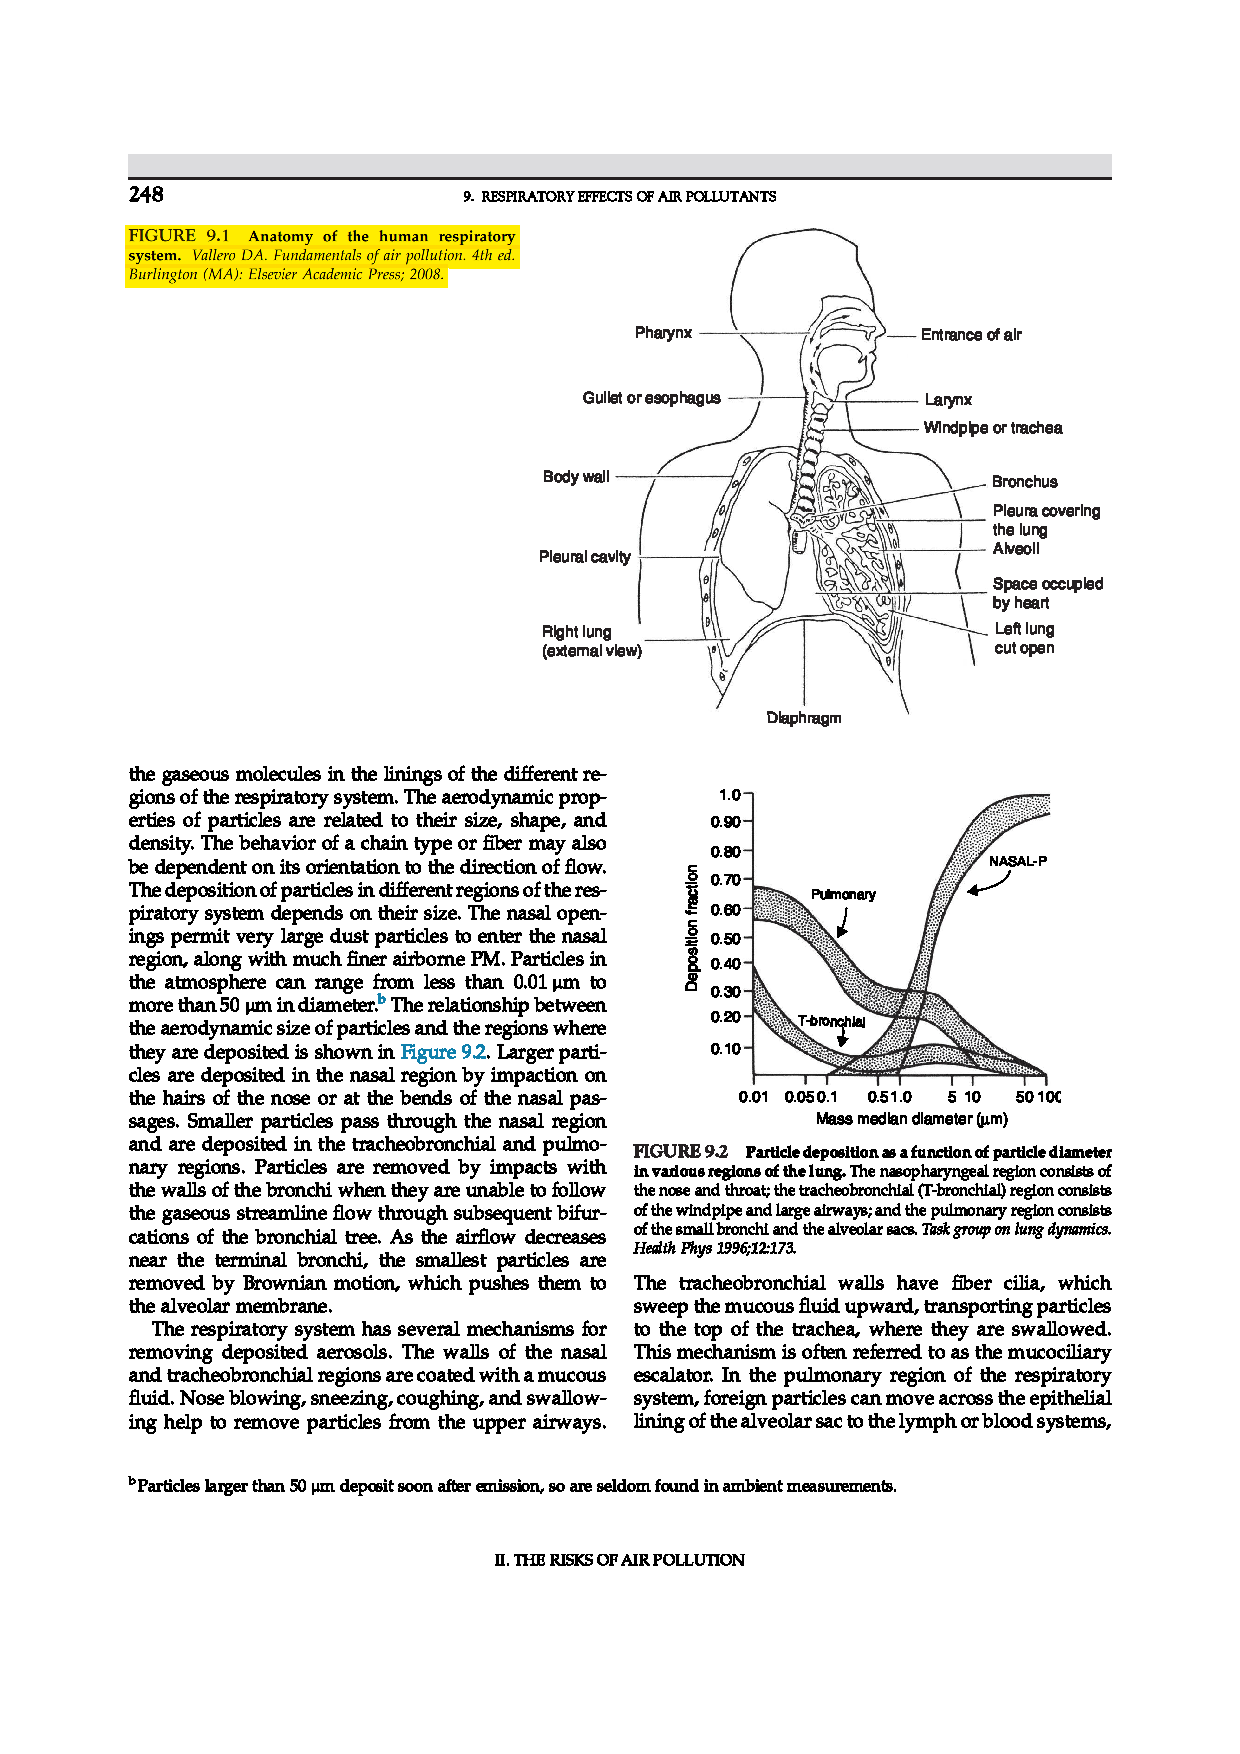
\includegraphics[clip,%
    trim=9.1cm 17cm 2.1cm 5cm,%
    width=.8\textwidth]{img/pdf/respiratory_system.pdf}
    \caption{Annotated anatomy of the respiratory
    system~\cite{Vallero2014}.}
    \label{fig:respiratory_system}
\end{figure}

The respiratory system has several (imperfect) mechanisms in place to
prevent particles from reaching the blood stream. Larger particles are
deposited in the nose, by impaction on the hairs and bends of the nose.
Smaller particles are immune to this first barrier, and manage to get to
the trachea and bronchi, where they are filtered also by impaction, this
time on the walls of the innumerable bifurcations of the bronchial tree.
The smallest particles are removed through Brownian motion, which ends
up pushing them against the alveolar membrane. Deposited substances are
then removed through the action of cilia in the pulmonary system's walls
or by coughing, sneezing or blowing one's nose~\cite{Vallero2014}.

While the body is quite efficient at filtering out particles from the
respiration process, the same cannot be said about gaseous pollutants.
Removal of these compounds can only be achieved through absorption,
which depends almost exclusively in the gases' solubility. High
solubility compounds are absorbed directly in the upper airways
(SO\textsubscript{2}, for instance), while less soluble gases (such as
O\textsubscript{3} and NO\textsubscript{2}) are absorbed in the lungs
themselves. Irritant gases trigger a variety of responses, in which one
can include sneezing, coughing or bronchoconstriction. These gaseous
compounds are then diffused through to the bloodstream or the lungs
themselves try to convert them into other substances via biochemical
processes. In some cases, this attempt to detoxify a pollutant can lead
to much more problematic circumstances. For instance, the lung is known
to active procarcinogenics, substances that are only carcinogenic after
being metabolized in a certain way~\cite{Vallero2014}.

Acute symptoms of \gls{AP} exposure are very varied, and range from mild
irritation to complete respiratory failure, depending mostly on level of
exposure and individual sensitivity to the chemical compound. One of the
most important acute manifestations of \gls{AP} exposure are encompassed
within the \gls{ALRI} group. There are several studies in which the
relationship between this issue and \gls{AP} is deducted and explained,
mostly in developing countries, and it remains as one of the major
causes for infantile death~\cite{CABI2019, UNICEF2013}. Children are one
of the most affected demographics by \gls{AP}~\cite{EEA2016}, and one of
the chief reasons for this is that the human respiratory system is till
developing in this stage of life.

In a 2016 review~\cite{Goldizen2016}, the authors searched the
literature for childhood adverse effects of \gls{AP}, with a particular
focus on respiratory problems. They have found evidence for a number of
respiratory complications and diseases that were previously reported in
the literature caused or exacerbated by \gls{AP}. Effects are many, and
vary immensely in nature, severity and affected populations. Short term
effects, like coughing and wheezing were found for the three types of
major pollutant and several others; several papers mention an
association between the occurrence of respiratory infections and
exposure to \gls{AP}, namely concerning \gls{PM} and \gls{no2}.  The
same review found reports of decreased lung function in children and
asthma exacerbation in children due to \acrlong{AP}. Moreover, a person
exposed to high levels of \gls{AP} during childhood are also more likely
to develop syndromes like \gls{COPD}, and to have exacerbated symptoms
of this disease. Finally, and perhaps more concerning, the carcinogenic
nature of several of the constituents of \gls{AP} leads to findings
relating the appearance of respiratory cancers to exposure levels during
childhood. Many of the conclusions of this review come from a
large-scale European effort called \gls{escape}, that intended to
investigate long-term health effects of \gls{AP} in Europe. \gls{escape}
was an \gls{fp7} initiative that ended in 2014.

\subsubsection{\acrlong{AP} and cardiovascular issues}%
\label{ssub:ap_and_cardiovascular_issues}

After being absorbed by the respiratory system, oxygen is distributed to
all cells of the body through the cardiovascular system. Air pollutants,
like particles and trace gases, are also capable of penetrating the lung
barrier and therefore share the same fate. There are several pathways
with which \gls{AP} and negatively affect the cardiovascular system. The
most immediate of which is probably an imbalance in the \gls{ans} caused
by direct inflammation and oxidative stress in the respiratory system.
The second most immediate pathway is systemic inflammation caused by
\acrlong{AP}. Finally, soluble \gls{AP} compounds in the bloodstream
also contribute to \gls{cvd} by increasing inflammation and oxidative
stress in the cardiovascular system~\cite{Brook2008, Vallero2014}.

The link between Air Pollution and cardiovascular effects started being
made during the twentieth century, given a series of incidents (like
London's 1952 killer-smog) that happened in the urban areas of
industrialized countries. Nowadays, \gls{cvm} has been shown to be
intricately connected to \gls{AP}. In fact, in a 2013 review indicated
that an annual increase of 10$\mu g / m^{3}$ in fine \gls{PM} and
NO\textsubscript{2} led to an increase of 11\% and 13\% respectively in
terms of \gls{cvm} and premature atherosclerosis, in spite of absolute
\gls{AP} concentrations were maintained below the European
policy-recommended thresholds. Road traffic exposure studies have
reported similar findings, with subjects having increased coronary
calcium scores~\cite{Bourdrel2017}.

Arrhythmia is one of the other cardiovascular issues that might be
caused by \gls{AP}. There is still some debate regarding whether or not
there is a causal relationship between the two, but there have been
several studies in which increased levels of \acrlong{AP} were
correlated with arrhythmia-related hospital admissions. Moreover, there
seems to be a correlation between low heart rate variability and
\gls{AP}, which is considered a marker for \gls{ans} imbalance and an
important risk factor for \gls{cvm}\cite{Bourdrel2017}.

The risk of stroke is also clearly exacerbated by the presence of
increased levels of \gls{AP}. In fact, it is currently thought that
\gls{AP} is responsible for about 29\% of the burden of stroke,
globally. Studies have shown that an increase of 5 $\mu g / m^{3}$ in
the annual \gls{PM}\textsubscript{2.5} concentration leads to a
remarkable 19\% increase in the risk of stroke, which was found to be
more significant in non-smokers. A positive correlation was also found
between gaseous pollutants (no\textsubscript{2}, CO and
SO\textsubscript{2}) concentration and the risk of stroke or stroke
mortality.

Short term effects of \gls{AP} on the cardiovascular system seem to be
predominantly the triggering acute coronary incidents. For instance, a
positive correlation was found between short term increases in \gls{AP}
and non-fatal myocardial infarctions.

\subsubsection{Gestational and developmental complications}%
\label{ssub:gestational_and_developmental_complications}

Mammals are in their life's most vulnerable stage while they are still
developing inside their mother's womb. This is the time when there is a
greater rate of tissue expansion and creation, creating an enormous need
for nutrients. These are supplied by the mother's blood, crossing the
placenta and reaching the fetus through its umbilical cord. High rates
of tissue formation and proliferation render the forming being unstable
and therefore more susceptible to the appearance of some kind of
morphological abnormality. At this time, there is no separation between
the mother's blood and the fetus, meaning that whatever chemical reaches
the progenitor's bloodstream also reaches the growing fetus. If the
mother is exposed, so is the fetus~\cite{Vallero2014}.

There are numerous chemicals that can affect the female reproductive
system, of which some are habitual components of \gls{AP}. They have
been associated to several highly adverse affects, and interfere with
such things as the processes by which the body is able to produce eggs,
or other processes that enable the formation of a single cell by the
union of the sperm and the egg (the zygote). After conception, \gls{AP}
has been known to reduce uterine nurturing capabilities, and hinder the
new being's development. Some of them are even teratogens, meaning that
they induce birth defects. Figure~\ref{fig:AP_in_utero} illustrates the
kind of defects that come with exposure, according to the time at which
the mother was exposed.

\begin{figure}[htpb]
    \centering
    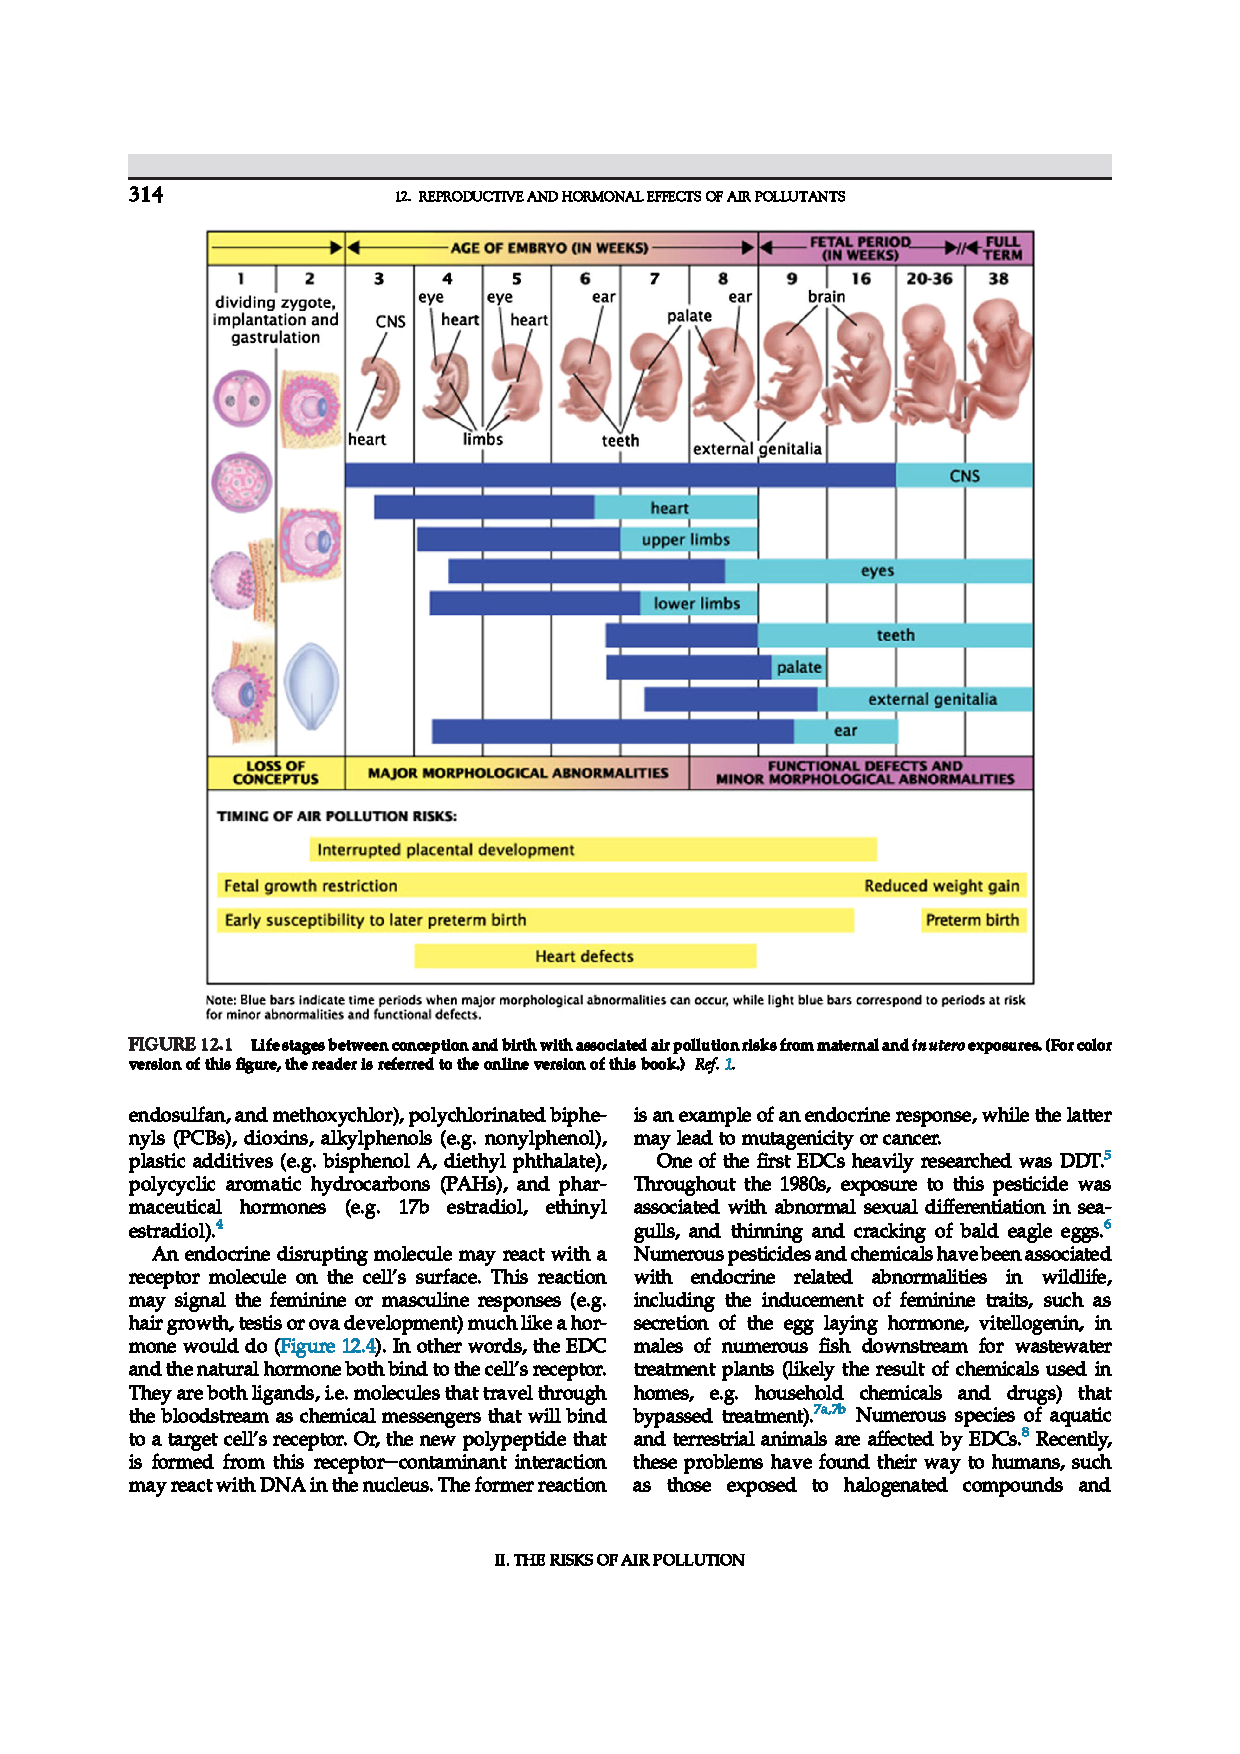
\includegraphics[clip,%
        trim=3.4cm 12.2cm 3.4cm 3.6cm,%
        width=0.8\textwidth]{img/pdf/development.pdf}
    \caption{Possible abnormalities caused by \gls{AP} exposure \emph{in
    utero}. Notice that time of exposure is of critical
    importance~\cite{Vallero2014}.}
    \label{fig:AP_in_utero}
\end{figure}

There are already several studies that correlate higher \gls{AP}
exposure levels to birth defects or the probability of negative
outcomes. For instance, in~\cite{Li2019}, researchers have studied the
association between \gls{AP} exposure levels (for the mother) and the
appearance of premature \gls{sga} by collecting more than 40000 births
in Changzhou Maternity (China) and studying the mother's typical
environment. This study has found a positive association between
\gls{sga} and exposure to \gls{PM}\textsubscript{2.5} in two or three
pollutants models of \gls{AP} (with \gls{no2} and \gls{so2}), during the
third trimester of gestation. Another, perhaps more comprehensive study,
was performed using Swedish data from 1997 to 2007, and found that there
was a positive association between \gls{o3} exposure and the appearance
of pre-eclampsia (a potentially deadly complication of pregnancy),
estimating that about 1 in 20 pre-eclampsia cases were caused by
\gls{AP}~\cite{Olsson2013}.

Besides uterine development compromises, birth defects and reproductive
difficulties, \acrlong{AP} has also been associated with hindrances to
the child's neurodevelopment. In a New York study was able to associate
lower levels of mental development at age 3, in African-American
children with valid prenatal \gls{pah} exposure data. In another study
from the neighboring Boston, \gls{AP} was associated with generally lower
cognitive test scores, even when correcting for several influencing
factors. On a different level, \gls{AP} was shown to produce significant
delays in the central conduction times of \gls{baep} tests in children,
indicating that there might be important repercussions of \gls{AP} to
vestibular and auditory development.

Although most other systems are affected by \gls{AP}, it does have a
particularly heavy toll on the respiratory development. This is because
the lungs are not completely developed at birth, and are only finished
in the late teens. The level to which \gls{AP} affects the respiratory
system development varies greatly with the staeg of life in which the
effect is produced, and severity is also very varied. Acute negative
effects range from respiratory death to chronic
cough~\cite{Vallero2014}. Moreover, childhood (and prenatal) exposure to
\gls{AP} has been associated with the emergence of conditions such as
\gls{COPD} and asthma.

\begin{figure}[htpb]
    \centering
    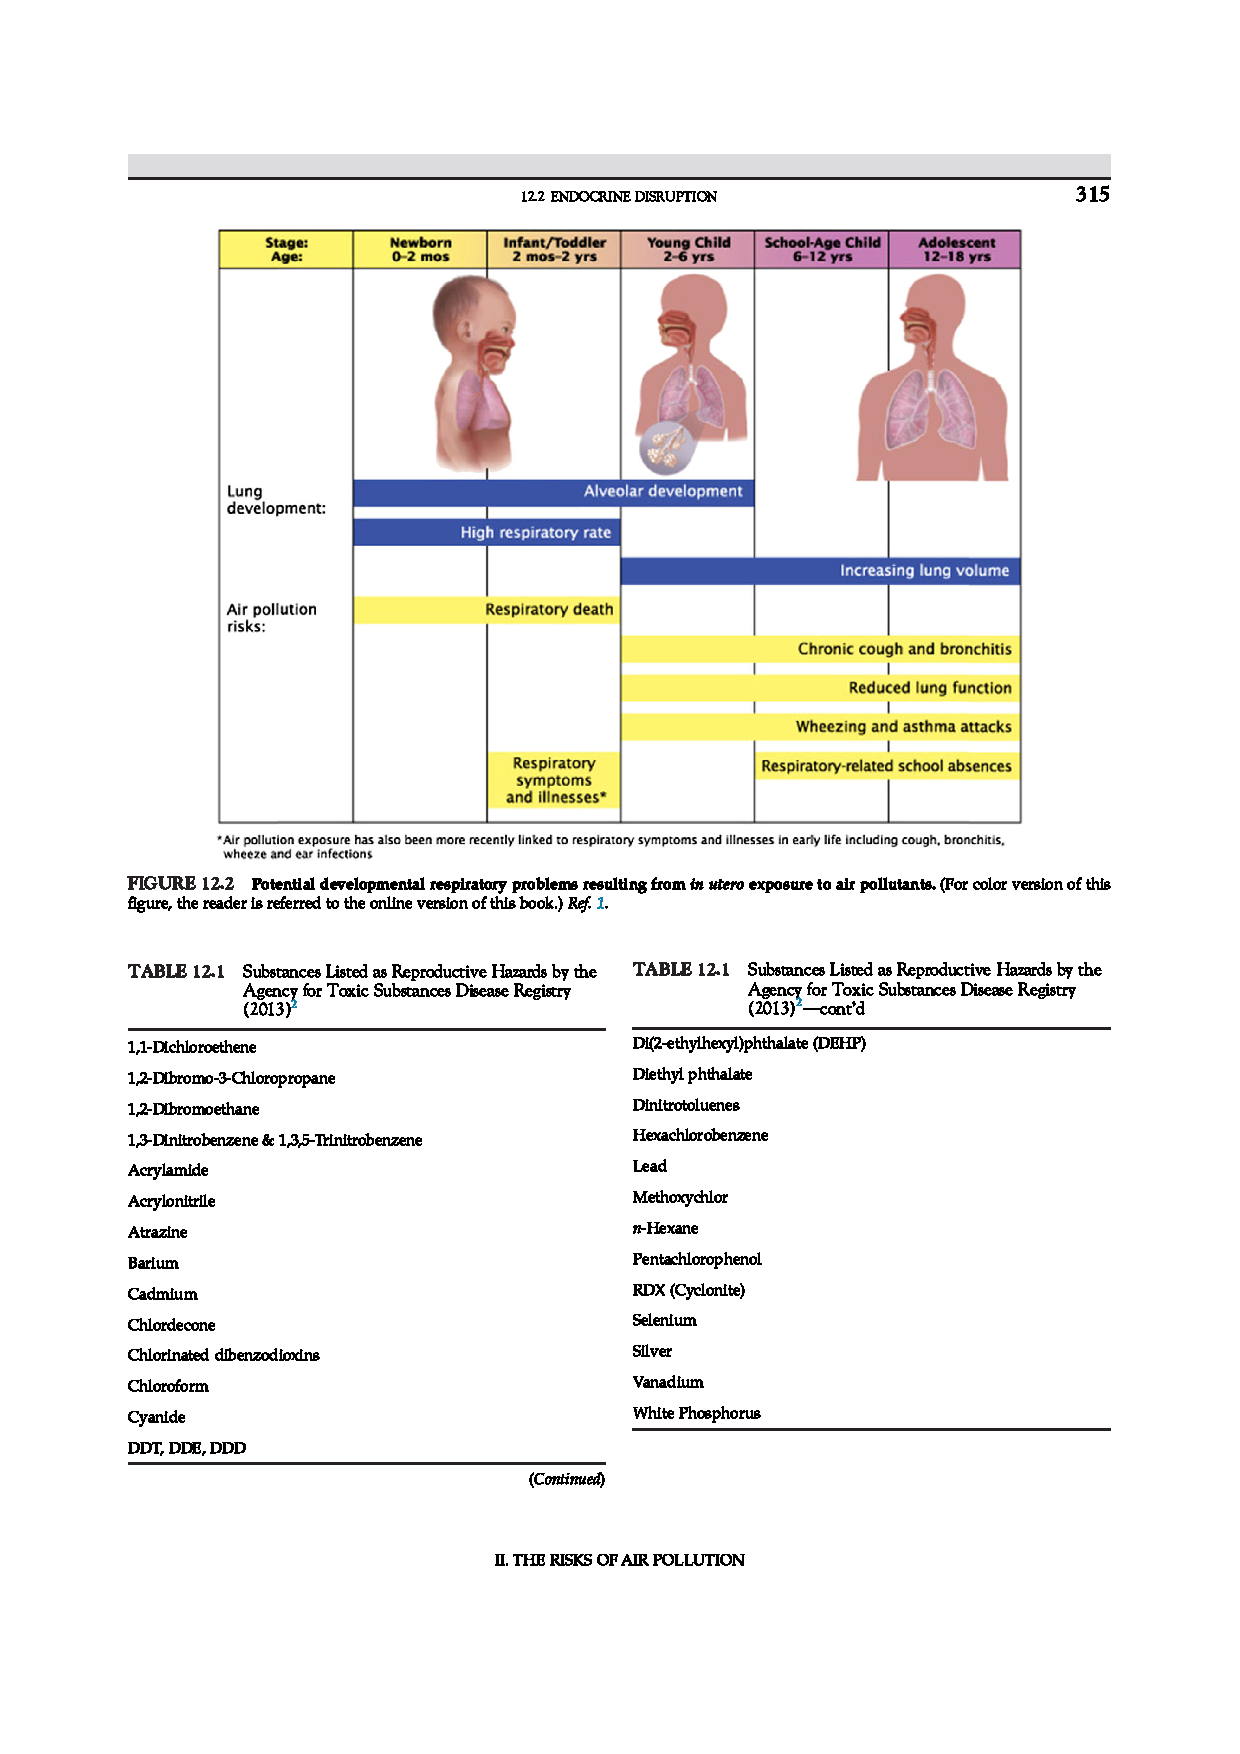
\includegraphics[clip,%
        trim=3.4cm 15cm 3.4cm 3.6cm,%
        width=0.8\textwidth]{img/pdf/lung_development.pdf}
    \caption{Developmental stages of the lung throughout life vs the
    risks of \gls{AP} exposure in each stage~\cite{Vallero2014}.}
    \label{fig:img/lung_development}
\end{figure}

\subsubsection{Neurological disorders}%
\label{ssub:neurological_disorders}

The brain and the \gls{cns} were one of the last to be included in the
range of organs that are affected by \gls{AP}. While the effects of
\gls{AP} on the respiratory and cardiovascular systems are quite broad
and include some "surprises", the fact that these systems were affected
by \acrlong{AP} was evident and expectable, given the type of exposure
these systems endure. The \gls{cns}, on the other hand, has a more
difficult to express relationship with \gls{AP}, and has required more
sophisticated methods to detect~\cite{Vallero2014, Genc2012}. It was in
the beginning of this century that the first connections between
\gls{AP} and the emergence of neurological disorders started to be made,
and from then on, we have progressed into thinking that not only are
they related, but also that \gls{AP} might be one of the key driving
forces in the onset of certain neurological diseases, including the most
dreaded of them all, Alzheimer's and Parkinson's~\cite{Genc2012,
DePradoBert2018, Calderon-Garciduenas2014}.

The reason why \gls{AP} is able to reach and damage the \gls{cns} is a
continuation (or even an extension) of the ways in which it affects the
cardiovascular system. By crossing the alveolar barrier into the
bloodstream, \gls{AP} acts as an oxidative stress source. As it can also
do in lung tissue, \acrlong{AP} creates some local proinflammatory
effects in the cardiovascular system, affecting the vascular endothelium
cells. This can lead to a systemic inflammatory status, which is
accompanied by the production of proinflammatory cytokines (a type of
message-protein that is used by organisms to trigger certain types of
response, like inflammation~\cite{Zhang2007}). Now, since blood vessels in the
brain are extremely responsive to this kind of message, their presence
can activate cerebral endothelial cells and disrupt the blood-brain
barrier~\cite{Genc2012}.

In 2018, a consortium of several Spanish universities and researchers
wrote a review detailing the until-then-published articles dealing with
the neurological implications of \gls{AP}~\cite{DePradoBert2018}. This
review identifies several articles that connect the long-term exposure
to \acrlong{AP} with adverse impacts on the brain and brain structures.
\emph{In vitro} and \emph{in vivo} studies,  focusing on traffic related
emissions and their effect on gray matter cells, have found that these
display significant alterations. On other studies identified by the
review, it was shown that white matter, the myelinated part of the
brain, is particularly sensitive to \gls{AP} and its volume is
significantly decreased both in the elderly and children, as consequence
of prolonged exposure to it. 

There are also several articles that show that there is an association
between exposure to air pollutants and impairments on brain function.
In Section~\ref{ssub:gestational_and_developmental_complications},  I
have already mentioned a study that was conducted in New York, and that
found that the children that they were using as subjects were found to
have measurable cognitive deficits in comparison with children of the
same age living in less polluted areas which are compatible with the
affected areas of the brain that were detected through neuroimaging
studies~\cite{DePradoBert2018}.

\subsection{\acrlong{AP} effects on ecosystems}%
\label{sub:ap_effects_on_ecosystems}
\todo[inline]{citations - vallero and lovett + european report}
The Earth is home to an almost unbelievable number of different
ecosystems. The ubiquitousness of \gls{AP} means that all of them are in
some way or another affected by this problem. In general terms, the
threat posed by \gls{AP} to any given habitat is a function of its
biodiversity, defined as the number of different living beings that
inhabit a certain environment (in all biological
kingdoms)~\cite{OxfordPress2020}. Living beings within an ecosystem are
like nodes in a graph, with many connections to any particular node.
More biodiversity corresponds to a greater number of nodes and an even
larger number of links,  which means that there is a greater probability
that some of those links become disrupted by \acrlong{AP} in some way.

Water based environments are greatly affected by \gls{AP}. Material
deposition on the surface of the water can have serious consequences in
terms of habitat conditions for holding life. In this regard, the most
important air pollutants are \gls{no2} and \gls{so2},  which
significantly decreases the water's pH. On its own, this represents a
major problem. The acidifying effects of nitrogen and sulfur deposition
became very pronounced in Scandinavia (among other places). Thousands of
this territory's lakes, once teeming with wildlife, became effectively
lifeless. Those that did not reach this point, have seen the number of
fish living on their waters dwindle to numbers from which there may be
no return~\cite{DeWit2015}. Sulfur and nitrogen depositions also enrich
surface waters, altering the solubility and other physical aspects on
the surface of the water, which in turn inevitably leads to disruptions
in species abundance and diversity. Moreover, indirect effects may also
take their tolls. For instance, \gls{o3} does not play any significant
role in the chemical behavior of a water body, but it can influence the
number of predators around this habitat, which will compromise the
predator-prey balance of the aquatic environment~\cite{Vallero2014,
Lovett2009}.

In terrestrial ecosystems, \gls{AP} effects are not smaller in
importance or complexity, and they are different for each type of being.
To the Flora, \gls{AP} can have a subtle to deadly effect, depending on
variables like pollutant chemical species, exposure time, or plant life
stage in which exposure happens. For instance, \gls{o3} is especially
poisonous to plants. Even small concentrations of this gas will cause
plant growth to decrease significantly. It enters the plant through the
stomata and reduces photosynthesis through increased oxidative stress.
Many times, although concentrations are not enough to outright kill the
plant, they are enough to make them more susceptible to other attacks
like pathogens, insects or environmental conditions. \acrlong{o3} is
commonly responsible for huge financial losses that come from the
diminished agricultural yields. And while it is true that due to several
policies, \gls{AP} is in a clear downward trend since the 1980s in urban
regions, it is also true that in many rural areas, these changes have
been smaller or non-existent, making these losses even more relevant.

Forests are among the most susceptible environments to \gls{AP}. They
suffer from the previously described mechanisms of \gls{AP} damage, like
acidic deposition, but also suffer from other, less direct pollution
risks. Emission of greenhouse gases can induce changes in humidity,
temperature, and general climate profile of a forest. The combination of
direct and indirect risks result in an exacerbation of both, leading to
more and more forest losses due to \acrlong{AP}. The damage done to
forests all around the world is especially problematic given the
biodiversity that these ecosystems contain within themselves.
Rainforests in particular are thought to contain more than half of the
world's terrestrial species. These species have many times adapted to a
particular kind of microhabitat which only exists in the specific
rainforest in which it lives. Changes in these specific conditions,
whether caused by \acrlong{AP} or any other cause, are leading to
alarming extinction rates in forests and rainforests globally.

Of course it is not only the flora that suffers with \acrlong{AP}.
Direct implications of \gls{AP} on animals approximate those that fall
upon humans. We are an animal species, after all. Our main difference is
the adaptation capabilities that our superior intellect grants us, which
allows us to escape more or less unscathed for a longer period of time,
and to combat what we cannot escape from in ways which are simply
unaccessible to other animal species. So, although \gls{AP} has direct
effects on all animals that are exposed to it, ecosystem damage and
eventual destruction remains the most perilous factor for this
biological realm~\todo{should I get another source on this problem? }.





\subsection{\acrlong{AP} Sources}%
\label{sub:ap_sources}

There are almost as many \gls{AP} sources as there are pollutants. The
first major division between these sources is whether they are natural
or anthropogenic. However, this separation is not always clear, as one
source can lead to another and boundaries become fuzzy within their own
context. The most prominent example of such is the case of accidental
fires. While they are most of the times classified as a natural source
of \gls{AP}, their origin lies most of the times in human activities. In
this section, I will present a selection of the most important naturally
occurring air pollutants and examples of how they have affected human
lives throughout the times. The selection itself does not intend to be
complete description of pollution sources, but rather paint a general
picture of the subject.

\subsubsection{Natural Sources of \acrlong{AP}}%
\label{ssub:natural_sources_of_ap}

Although people, governments and institutions tend to speak far more
seldomly of them than of their man-made counterparts, natural sources of
air pollutant are not only abundant, but also important. One of the main
natural sources of \gls{AP} are volcanic eruptions. These phenomena are
responsible for the emission of immense quantities of \gls{PM} and gases
such as \gls{so2}, \gls{h2s} and methane. Depending on the type of
volcanic eruption, the emitted cloud of gas and \gls{PM} can remain
airborne for long periods of time, even disrupting modern life at times,
namely in what concerns air travel. The last eruption to happen in
Portuguese soil took place in the remote Azorian island of Faial. In
September 1957, the Earth shook almost continuously for around two
weeks. Finally, on the 27\textsuperscript{th}, 100 m Northeast the
Capelinhos islands, the sea was seen to boil and project vapor and
volcanic material hundreds of meters into the air. In the following
hours, the underwater volcano finally exploded, emitting large
quantities of volcanic ash and gases into the atmosphere. The phenomenon
lasted for more than a year, and the final ejection of lava took place
in October 1958 (see Figure~\ref{fig:capelinhos1957}). The eruption had
a significant social impact, in addition to its ecologic importance. In
the end, 40\% of Faial's population left the island as a
result~\cite{Vallero2014, TSF2017}.

\begin{figure}[htpb]
    \centering
    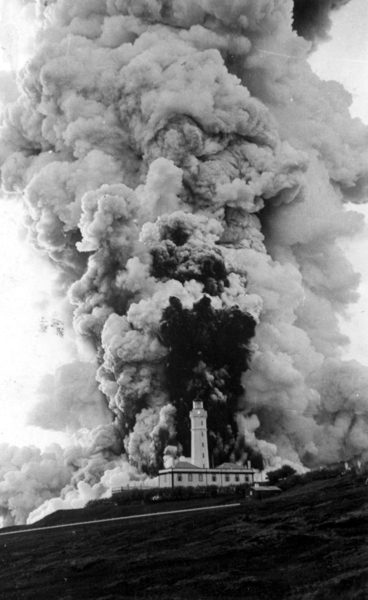
\includegraphics[width=0.8\linewidth]{img/jpg/capelinhos1957.jpeg}
    \caption{Dramatic photograph depicting the Capelinhos' lighthouse,
    half a kilometer from the eruption site, surrounded by a cloud of
    ash \gls{PM}, volcanic gas and water vapor with more than 1km in
    height\cite{TSF2017}.}
    \label{fig:capelinhos1957}
\end{figure}

Oceans are also a significant source of \gls{AP}. Aerosol particles of
salt are continuously emitted from these large masses of salt water,
which damage many human created structures, namely metallic
constructions. In certain parts of the world, another important source
of \acrlong{PM} (especially because of its consequences in the
inhabitants' daily life) are dust storms. The most famous of these
events, and one of the most deadly storms in the recorded history of the
US territory was the infamous \emph{Black Sunday} dust storm. Starting
on Palm Sunday, 14 April, this sky-blackening dust storm punished the
peoples from the panhandles of Texas and Oklahoma, burying entire houses
(see Figure~\ref{fig:dust1935}) under the dust and destroying the
livelihoods of thousands of Americans. Dust storms were an important
part of the US history during the 1930s and led to the creation of the
Soil Conservation Service, a branch of the US Department of
Agriculture~\cite{Vallero2014,Agriculture2012, Reis2008}.


\begin{figure}[htpb]
    \centering
    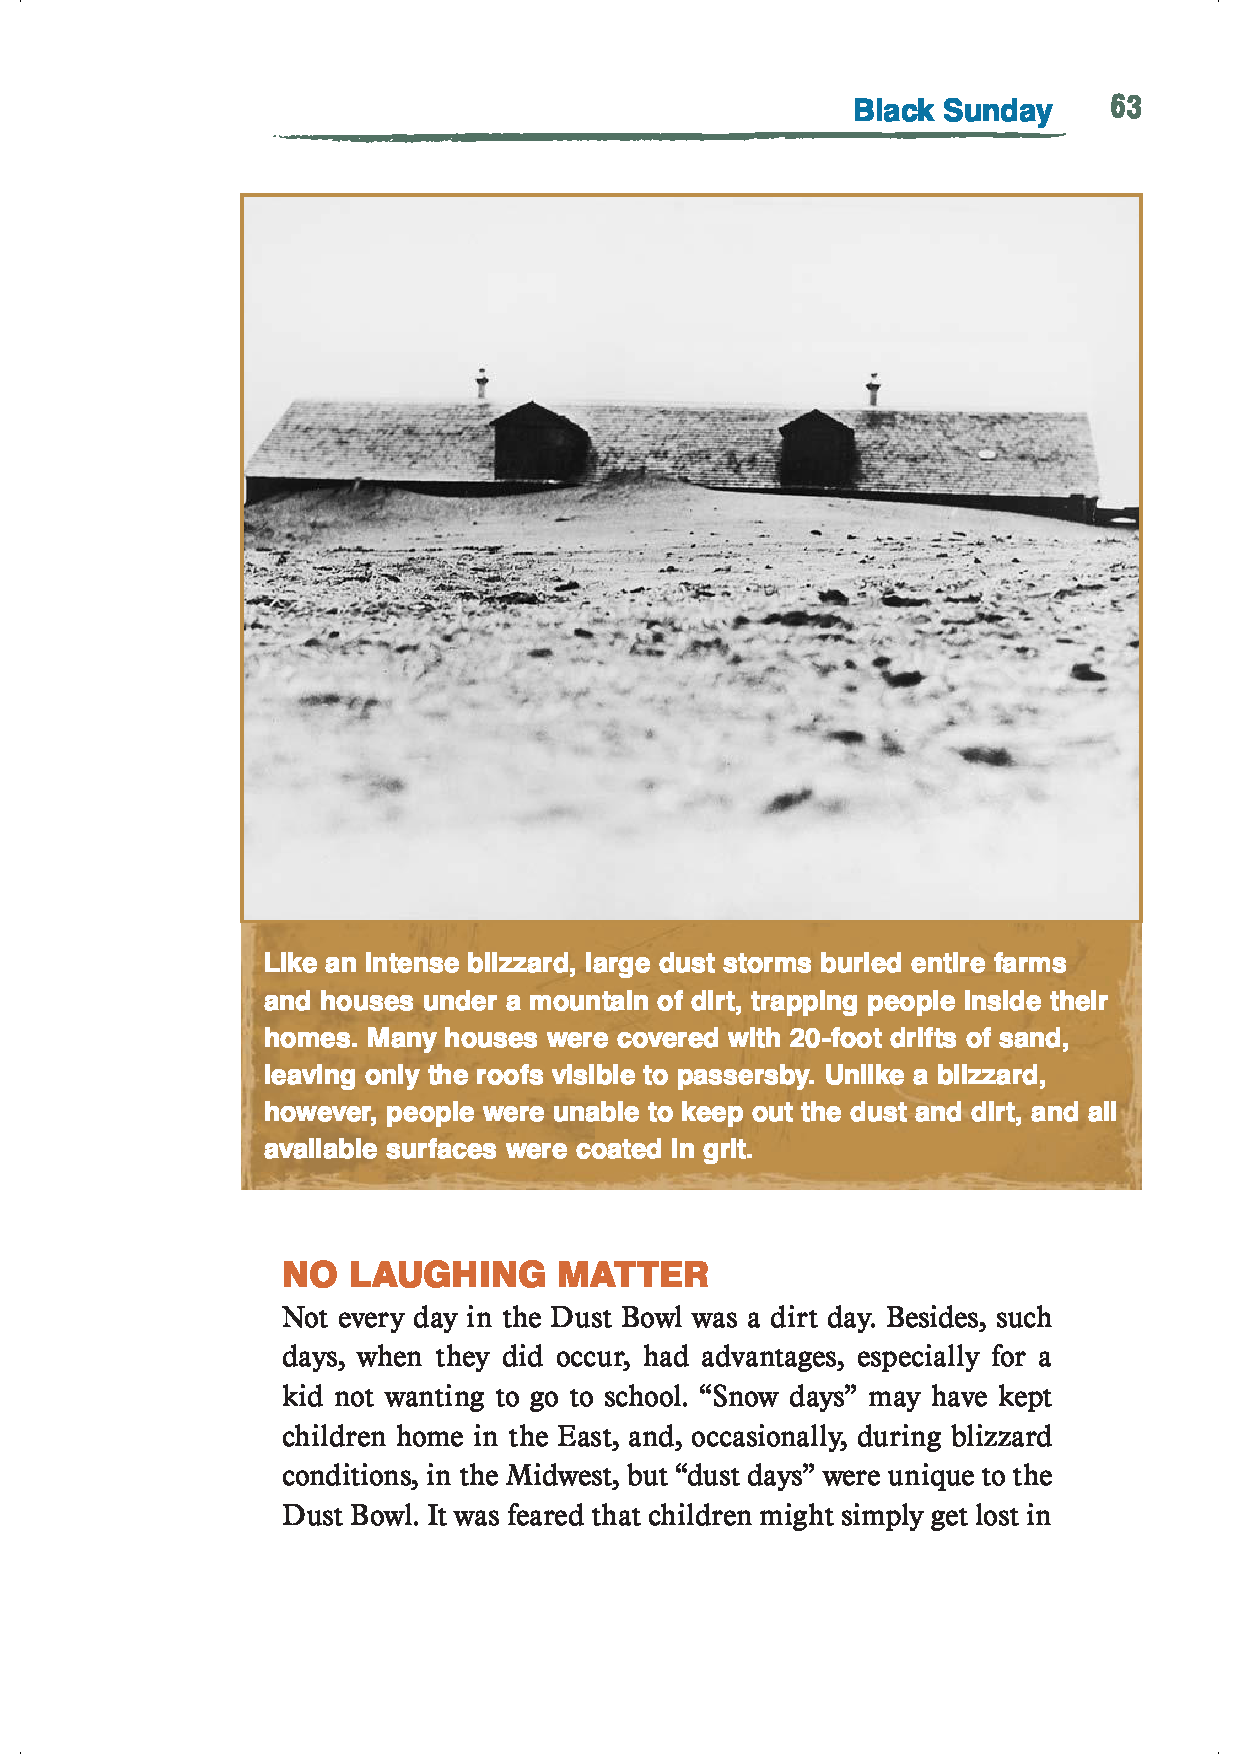
\includegraphics[clip,%
        trim=4.3cm 15cm 2cm 3.6cm,%
        width=0.8\textwidth]{img/pdf/dust.pdf}
        \caption{House almost completely buried by the Black Sunday dust
            storm. Several houses were entirely swallowed during this
            storm, trapping people inside, as if a big blizzard had hit
            them. Unlike a blizzard though, there was nothing anyone
            could do to keep the dirt outside, and all surfaces were
            covered black~\cite{Reis2008}.}
    \label{fig:dust1935}
\end{figure}

Fires are also one of the largest sources of natural air pollution in
the world. The uncontrolled burning of organic matter that is a large
forest fire creates a large quantity of air pollutants that range from
smoke to unburned (or partially burned) hydrocarbons, nitrogen and carbon
oxides, and ash particles. Besides the obvious dangers of this kind of
burnings for human life and activities, forest fires can also cause
indirect damages, such as disruptions in supplies and travel due to
reduced visibility~\cite{Vallero2014}.

Trees and forests in themselves are also responsible for a certain
quantity of air pollution. Although they have the main part in the
carbon dioxide conversion into oxygen, through photosynthesis, plants
and trees are still the largest emitters of hydrocarbons in the planet,
as attested by the blue haze that is visible on top heavily forested
areas, resulting from chemical reactions between \gls{VOC}s produced by
the trees. This counter-intuitive fact was in the origin of the infamous
Ronald Reagan speech in which he "blamed" trees for much of \gls{AP}, in
a time when anthropogenic \gls{AP} was at its apogee in the US and
Europe.Plants are also the emitters of another kind of \gls{PM}, which
is of particular importance both to themselves and humans, which are the
pollens. This is a bio-aerosol - a type of aerosol that is or was part
of a living being - associated with a number of
diseases~\cite{Vallero2014}.

Finally, I will discuss Radon gas. This is a natural occurring
radioactive gas that is part of the radiative decay of Uranium present
in all rocks. Although chemically inert, Radon is radioactive and, as
all radioactive substances, emits particles when it decays. Although
present virtually everywhere, outdoor concentrations of Radon are
typically too small to cause any problems. The problem with this gas
comes essentially from indoor concentrations, namely at home. Being a
gas, Radon is able to enter people's houses, exposing the inhabitants.
Prolonged exposure to Radon gas is the second biggest cause of lung
cancer and authorities estimate that between 3 and 14\% of lung cancer
cases are caused by this gas. In Portugal, Radon concentrations were
found to be below the European prescribed limit in two thirds of the
houses in a 2001 study, but in 17\% of the cases, concentrations were
not only above this limit, but also over the highest tolerable
limit~\cite{Vallero2014, WorldHealthOrganization2016, ProTeste2003}.


\subsubsection{Anthropogenic Sources of \acrlong{AP}}%
\label{ssub:anthropogenic_sources_of_ap}

\acrlong{AP} that originates from human activities is called
anthropogenic. Since the first industrial revolution, mankind has been
using more and more resources to fuel our progress and continuously
improving way of life. Of course, the consumption of natural resources
has some unpleasant and sometimes dangerous consequences. The most
important of which, looking from the lens of this thesis, is the
incredible increase in the levels of \gls{AP}. If one had any doubts
whatsoever, all it would take would be a look into the atmospheric
\gls{co2} concentration chart (Figure~\ref{fig:co2_concentration}) from
a few centuries back to the current day to completely dissipate them.

\begin{figure}[htpb]
    \centering
    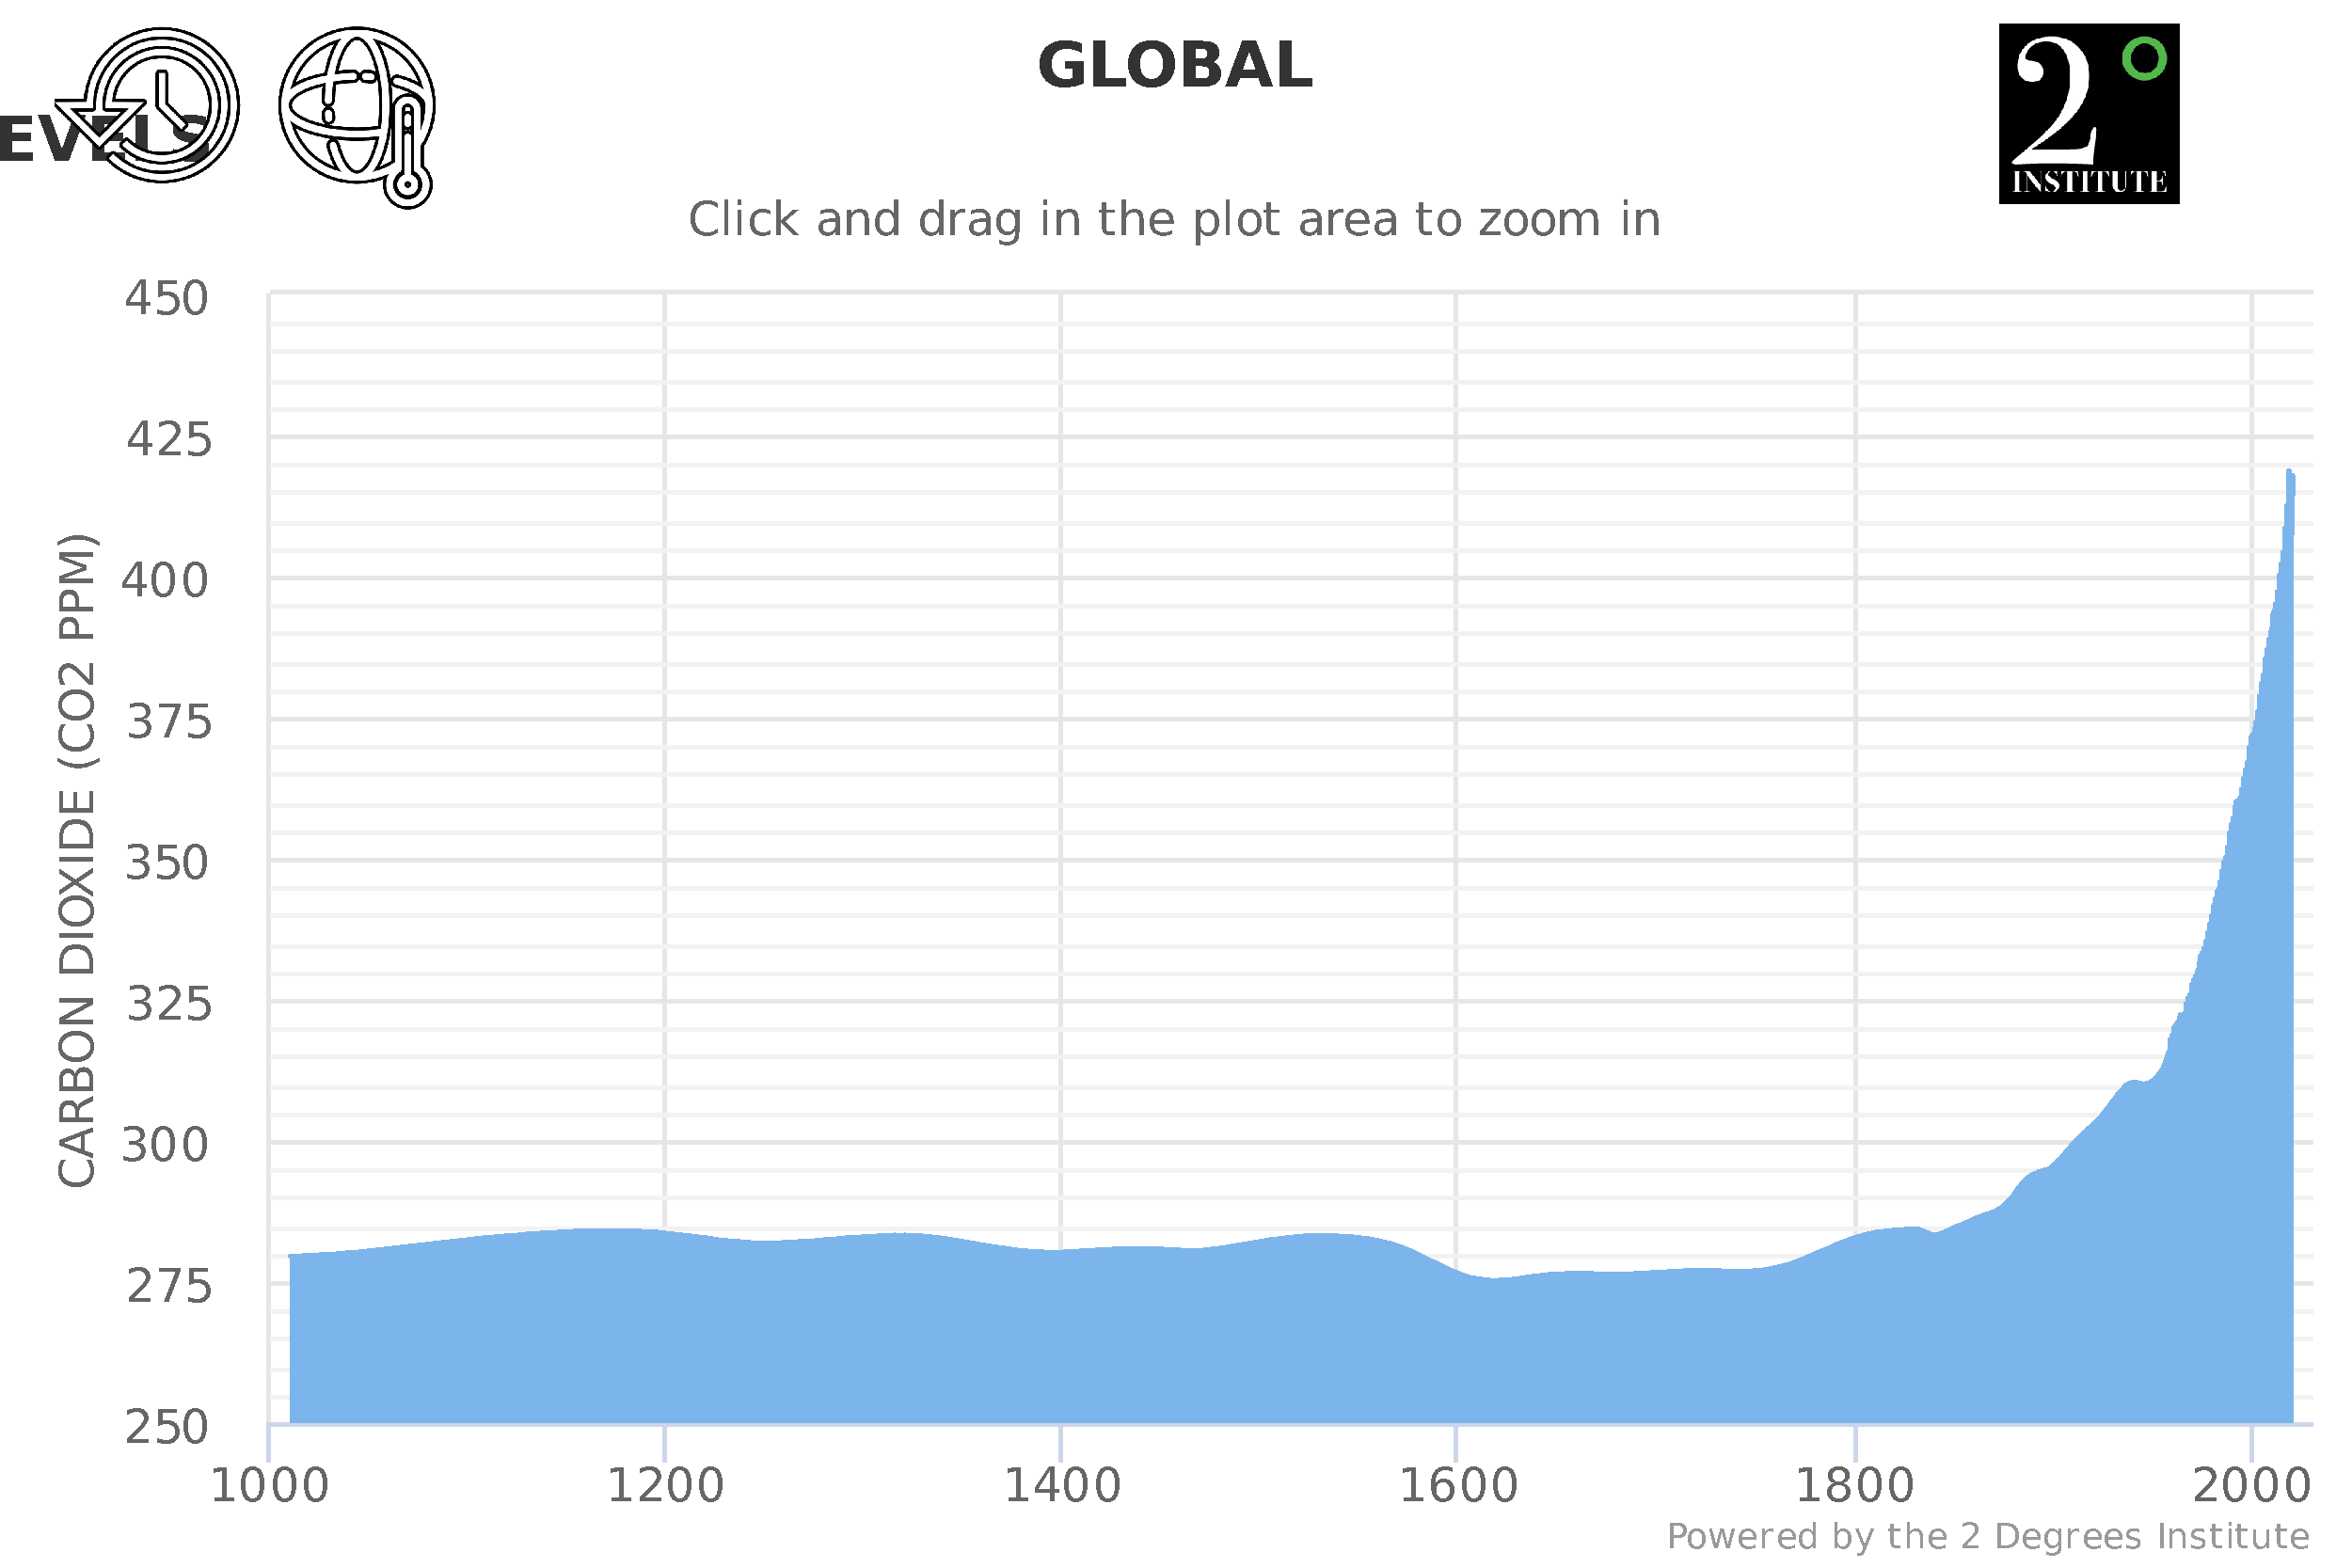
\includegraphics[clip, % left, bottom, right, top
                     trim=0cm 1cm 0cm 4.5cm,%
                     width=0.8\linewidth]{img/pdf/co2_ice_cores.pdf}
                     \caption{\gls{co2} atmospheric concentrations since
                         the year 1000. Note the seemingly exponential
                         increase since the 1800s. Plotted and published
                         by the 2 Degrees Institute~\cite{co2levels2020}
                         with data from ice cores~\cite{Etheridge} and
                         in situ monitors~\cite{Tans}.}
    \label{fig:co2_concentration}
\end{figure}

There are literally hundreds of sources of \gls{AP}, but it is possible
to categorize them into 4 main \emph{families}: industrial processes,
energy (includes transportation), agriculture and forestry, and waste.
Of these 4 broad categories, as displayed in
Figure~\ref{fig:anthropogenic_pollution_categories}. The most prominent
is without a doubt the energy sector, although we also have to bear in
mind that any and all combustion used in the other sectors is counted as
energy production~\cite{InternationalAgencyforResearchonCancer2016,
CABI2019}.\todo{table with major pollutants?}

\begin{figure}[htpb]
    \centering
    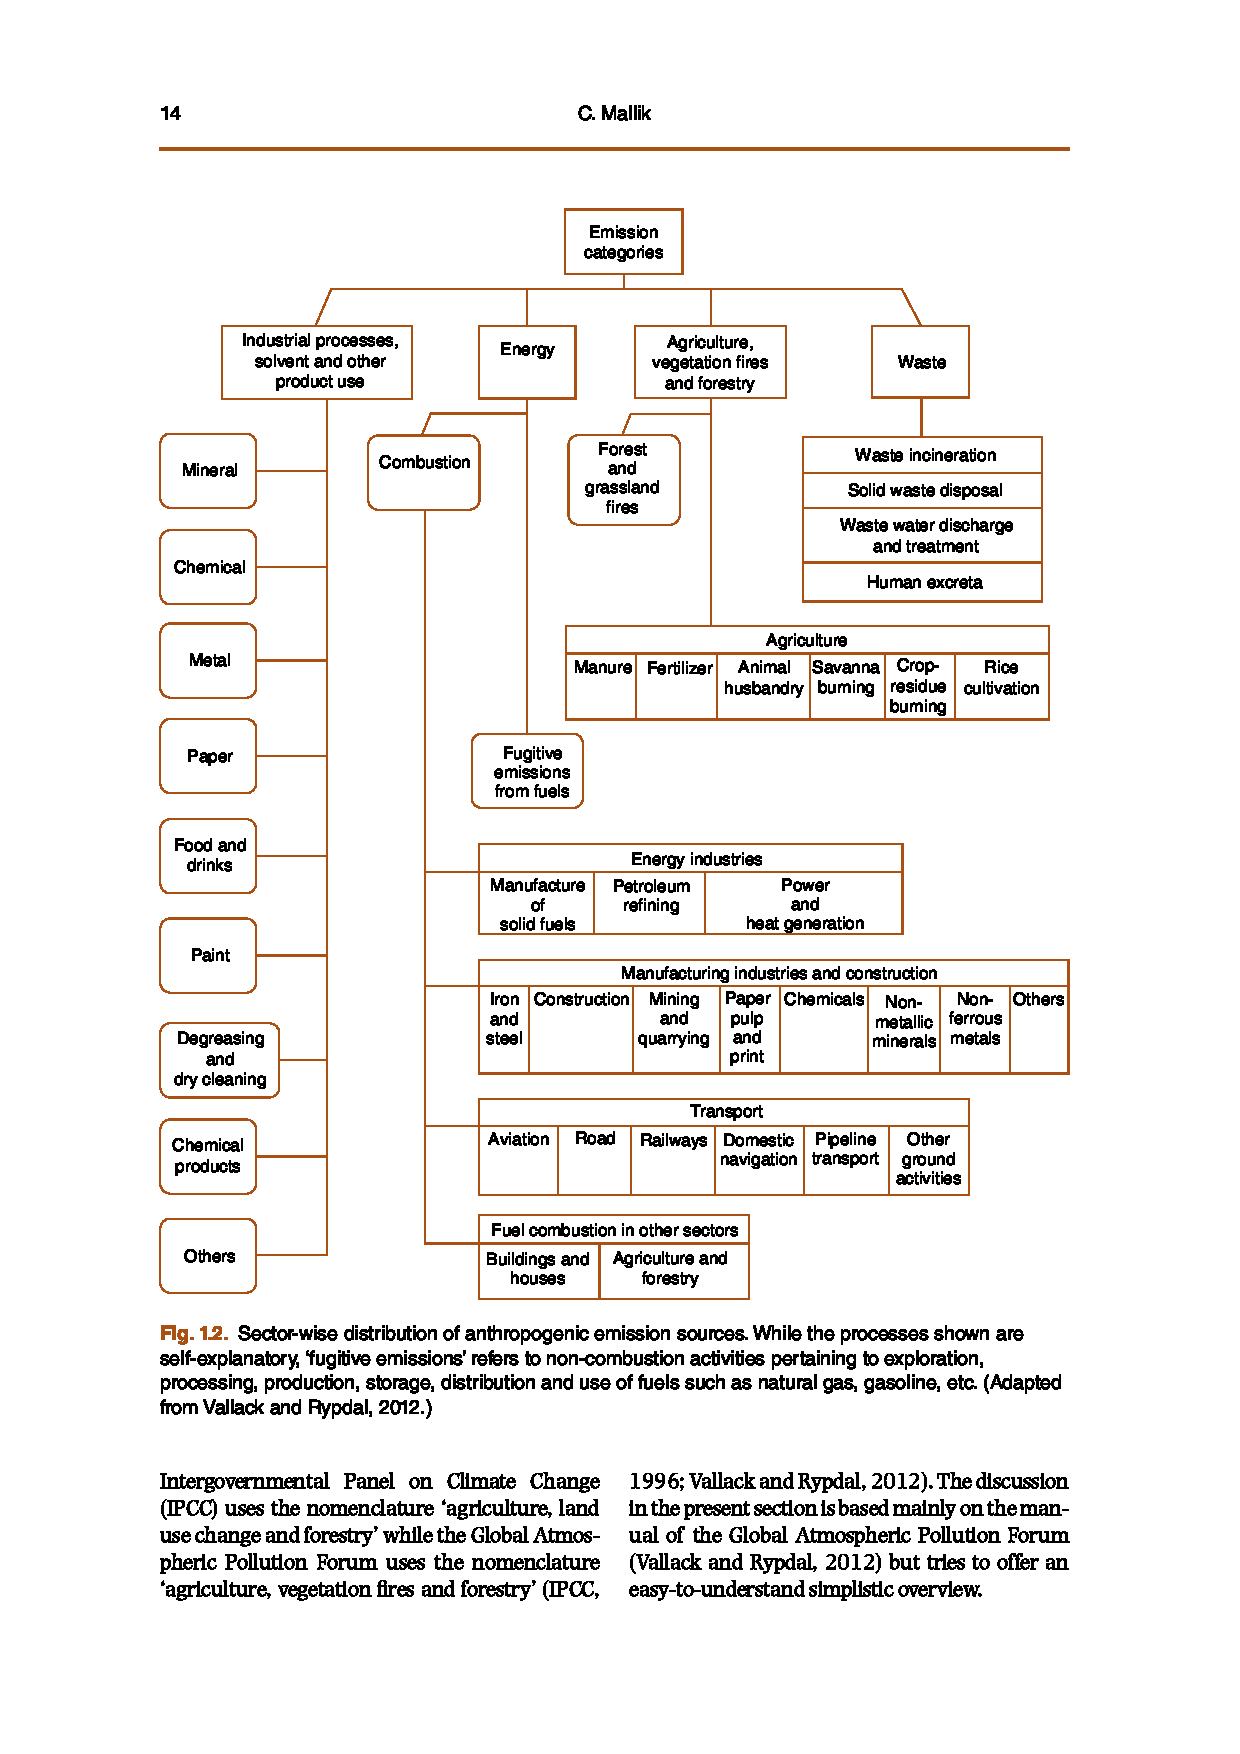
\includegraphics[clip,% left, bottom, right, top
        trim=2.3cm 7.3cm 2.3cm 2.6cm,%
        width=\textwidth]{img/pdf/pollution_sources.pdf}
    \caption{Schematic presentation on the sources of anthropogenic
    pollution and its categorisation according to the IPCC. Adapted
    from~\cite{CABI2019}}
    \label{fig:anthropogenic_pollution_categories}
\end{figure}

From 2002 to 2011, fossil fuel combustion has been responsible for an
average of 8.3 petagrams of carbon per year. This truly gigantic carbon
footprint is in its majority explained by the worlds energy needs, which
are ever increasing up to now. In 1990, total energy demand was situated
at 356 quadrillion \gls{btu}, having grown to 410 quadrillion \gls{btu}
in 2010. In 2020, energy demand estimates are located at 600 quadrillion
\gls{btu}, of which almost a quarter was expended by
China~\cite{CABI2019}.

It is important that we focus a little bit more on the Chinese case. It
is now somewhat near commonsense to regard China as the factory of the
world, and this of course is tied to Chinese energy consumption and
production. On the same line of reasoning, this must mean that in some
way, the country's energy expenditure is connected to the amount of
financial resources that it produces, the \gls{gdp}. Looking at the
plots in Figure~\ref{fig:china_energy}, one can see that all these
numbers are highly correlated. When we ponder on the case of Chinese
\gls{AP}, and wonder why has this problem not been addressed previously,
given its imposing dimensions and growing importance, one must take into
account that, given the indirect importance of \gls{AP} on Chinese
people's gains, it is highly likely that the country's governments will
be reluctant to decrease it in any expedient form~\cite{CABI2019, IEA,
WorldBank}.

\begin{figure}[htpb]
    \centering
    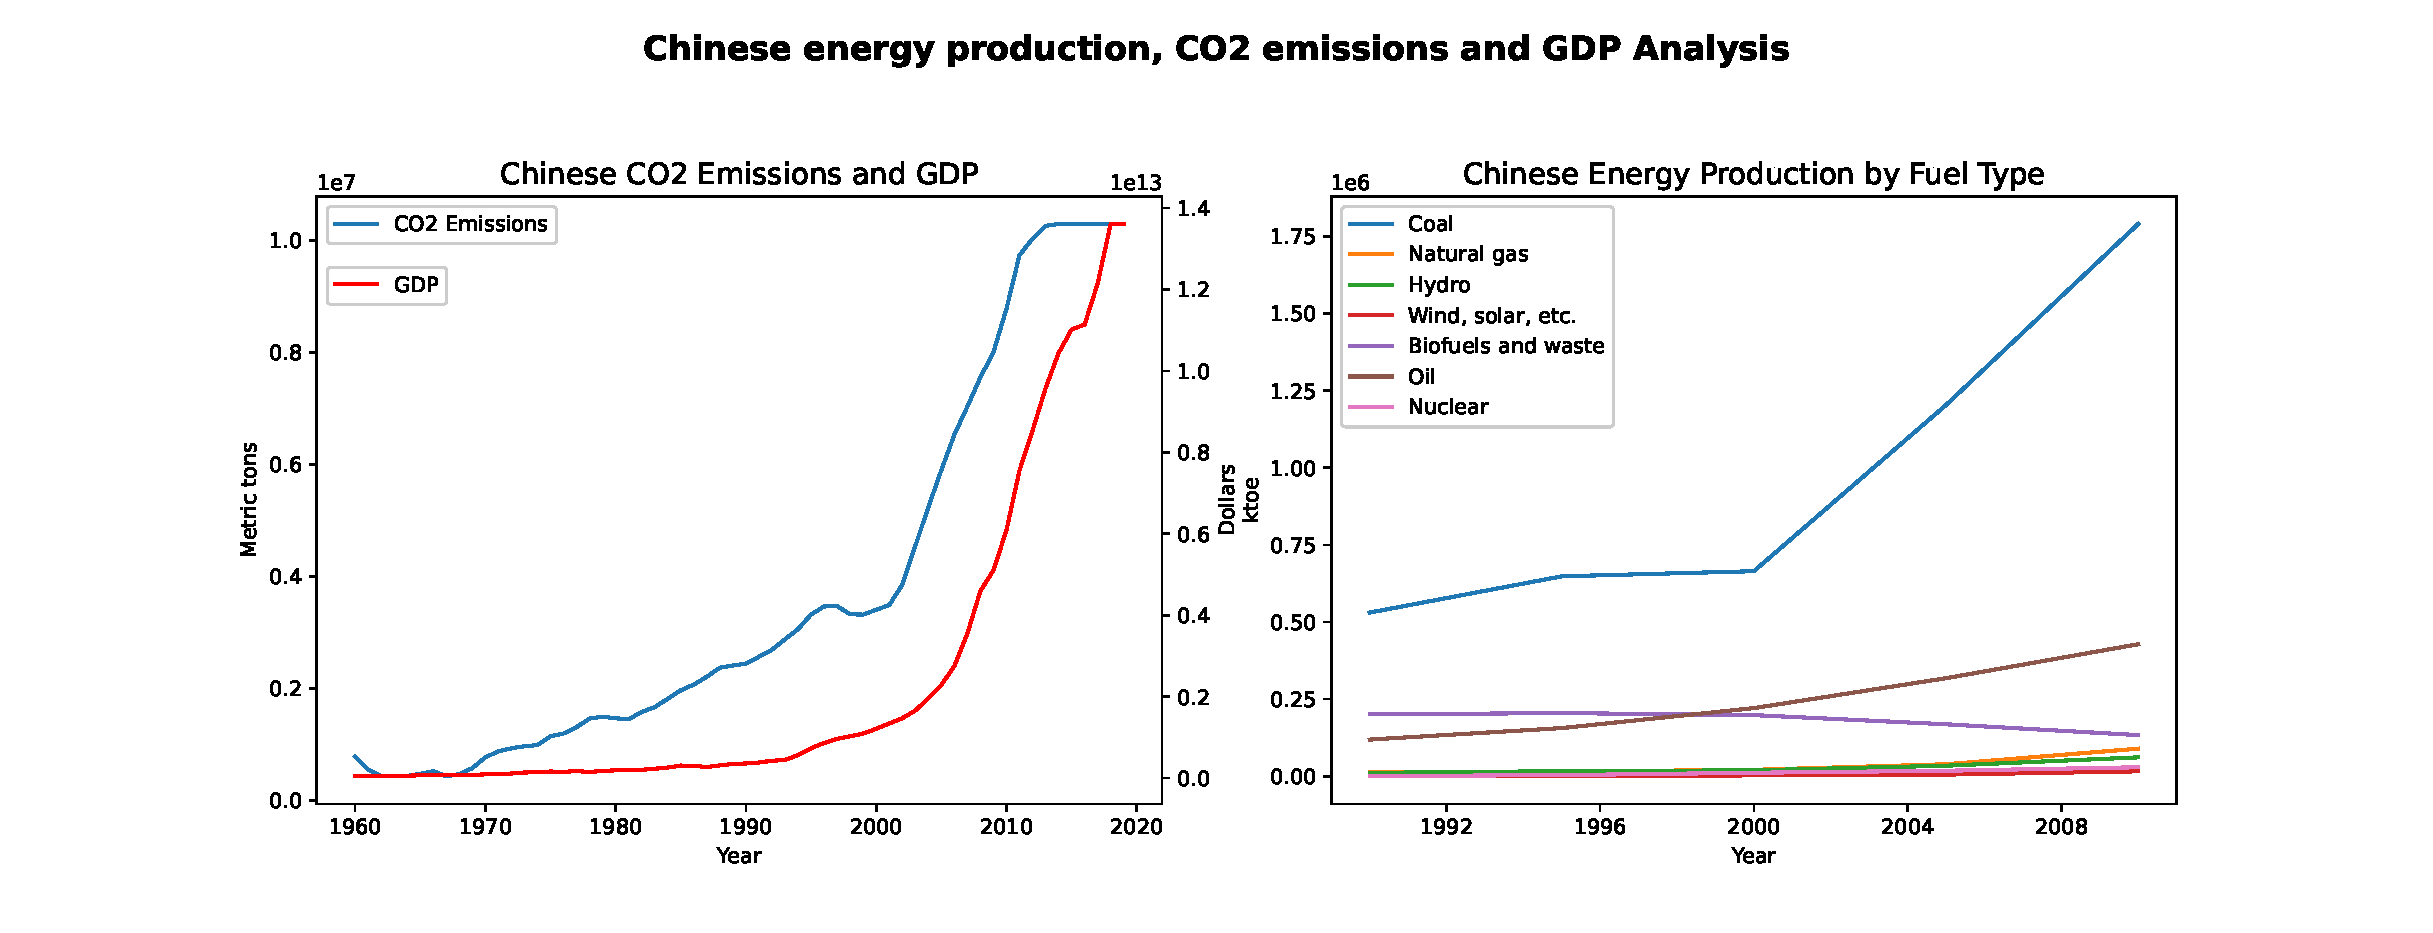
\includegraphics[width=\linewidth]{img/eps/energy_co2_gdp.eps}
    \caption{Chinese energy production, \gls{gdp} and \gls{co2}
    emissions.  Data collected from the World Bank and International
    Energy Agency websites~\cite{WorldBank, IEA}}
    \label{fig:china_energy}
\end{figure}

Another important conclusion that we can take from the plot in
Figure~\ref{fig:china_energy} is that China has a large and historical
dependence on the use of coal as fuel for energy production. This adds
to the problem described in the above paragraphs, as coal is the single
most damaging fossil fuel available. Not only does China get most of its
energy from coal burning, but is also responsible for more than half of
the worlds production and consumption of this substance (see
Table~\ref{tab:global_energy_consumption}).


\begin{table}[htpb]
    \centering
    \small
    \caption{Global energy production, divided according to the fuel
    used to obtain it and the production country.}
    \label{tab:global_energy_consumption}
    \begin{tabularx}{\textwidth}{lXXXXX}
    \toprule
    \textbf{Country} & \textbf{Liq. Fuel} &
    \textbf{Coal} & \textbf{Nat. Gas} &
    \textbf{Renew.} & \textbf{Nuc.} \\ 
                    &\textbf{\tiny{(M barrels /
    day)}}&\textbf{\tiny{(BTU)}}&\textbf{\tiny{(T cu.
                    ft)}}&\textbf{\tiny{(BTU)}}&\textbf{\tiny{(b kWh)}}\\\midrule
    \textbf{China} & 10,6 & 80,6 & 5,1 & 10,6 & 93 \\
    \textbf{USA} & 18,5 & 17,3 & 25,5 & 7,8 & 769 \\
    \textbf{Europe} & 14,4 & 12,5 & 17,9 & 11,7 & 837 \\
    \textbf{Middle East} & 16 & 0,1 & 14,8 & 0,2 & 1 \\
    \textbf{India} & 3,6 & 12,6 & 2,1 & 3,5 & 30 \\
    \textbf{Russia} & 3,4 & 4,5 & 15,7 & 1,7 & 166 \\
    \textbf{Africa} & 3,5 & 4,3 & 2,7 & 4,7 & 12 \\
    \textbf{Brazil} & 3,3 & 0,5 & 1,1 & 6,8 & 15 \\
    \textbf{World} & 91,4 & 153,9 & 120,8 & 63,7 & 2345 \\ \bottomrule
    \end{tabularx}
\end{table}

\gls{ice} are the single most important means for powering human
transportation. Almost every vehicle in the world uses a kind of
\gls{ice}. These motors operation is an application of the Otto cycle,
in which the chemical energy in the fuel is converted to mechanical
energy. These engines are as ubiquitous as the fossil fuels that have
powered them since the beginning of the automobile revolution, in the
early 20\textsuperscript{th} century. Fossil fuels have several features
that make them ideal to power our vehicles. Their energy density is
generally high~\todo{citation and examples}, they are incredibly safe to
manipulate and use, and fossil fuel infrastructure can be found in
almost every far corner of the Earth. However, using them releases a
number of gaseous and particle-condensed side products into the
atmosphere, and this makes traffic one of the most important sources of
\gls{AP}. For instance, traffic pollution is the main responsible for
human exposure to \gls{nox} gases. Without countermeasures, gasoline
\gls{ice} equipping passenger vehicles emit around 1.8 g/km of these
gases, while diesel emits 2.8 g/km and \gls{gpl} around 2.1 g/km. On
heavy duty engines, like on trucks and tractors, these figures skyrocket
to 14.7 g/km for diesel engines and around 5.1 g/km for
\gls{gpl}~\cite{CABI2019}.

Energy production (including transportation) is clearly the single
largest contributor to global \gls{AP}. This does not mean that other
human activities do not pollute or produce air pollutants. Pollutant
contributions from the industry, the agricultural activities and waste
disposal are also non-negligible. In fact, industries around the world
are responsible for the production and emission of all the criteria
pollutants. It is important to single out one particular activity, which
is the burning of forest for land-use changes. \gls{co} emissions for
this purpose are very high due to the nature of the burning material,
which emits more than 50 times more \gls{co} than fuel or
coal~\cite{CABI2019}.

\subsubsection{The European Case}%
\label{ssub:the_european_case}

Europe has for long been on the forefront of the fight against \gls{AP}
emissions. The European Union has put in place a number of policies
aiming at cutting (or even eliminating) emissions of human health
compromising pollutant components. Few places in the world have been so
demanding regarding their environmental practices, and numbers are a
clear reflection of these adaptation efforts. In their 2019 report, the
\gls{EEA} state that European emissions have globally declined, and have
been declining since at least the year 2000. Moreover, and in contrast
with China's case, the \gls{gdp} does no seem to be connected to
\gls{AP} emissions. As can be seen in
Figure~\ref{fig:european_emission_trends}, emissions are decoupled from
economic growth, as there are now less emissions per \gls{gdp} unit than
before~\cite{EEA2019}.

\begin{figure}[htpb]
    \centering
    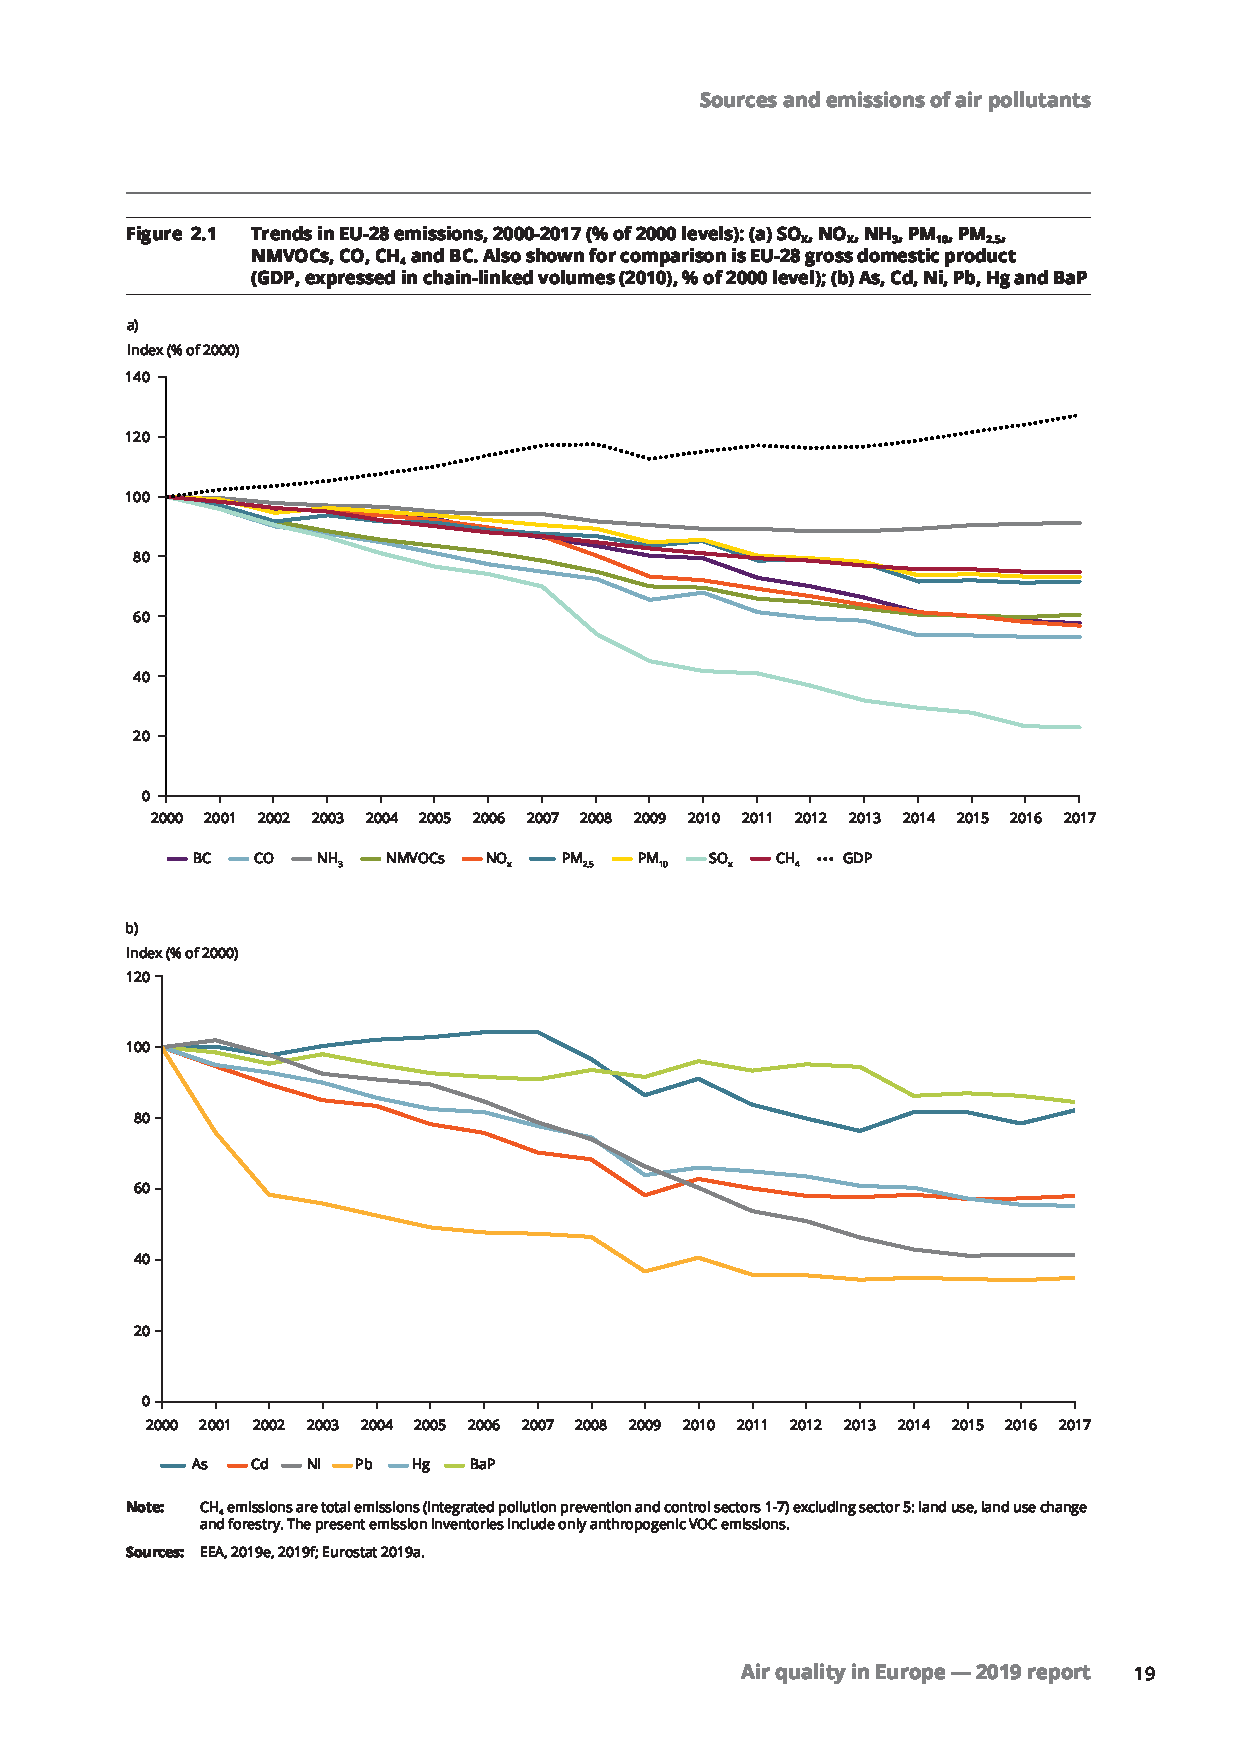
\includegraphics[clip,% left, bottom, right, top
        trim=0cm 15cm 0cm 5.8cm,%
        width=\textwidth]{img/pdf/european_emission_trends.pdf}
    \caption{General trends for European emissions. Data presented in \%
    emissions of year 2000. Note the downward global trend in pollutant
    emissions, and its decoupling with the European GDP~\cite{EEA2019}.}
    \label{fig:european_emission_trends}
\end{figure}

If one extends this analysis further, and separates emissions by using
their origin, the trends are approximately the same: except for
\gls{nh3} (a side product of agricultural activities) a clear reduction
is present in all sectors. These results can be seen in
Figure~\ref{fig:european_emissions_by_sector} and were presented
in~\cite{EEA2019}.

\begin{figure}[htpb]
    \centering
    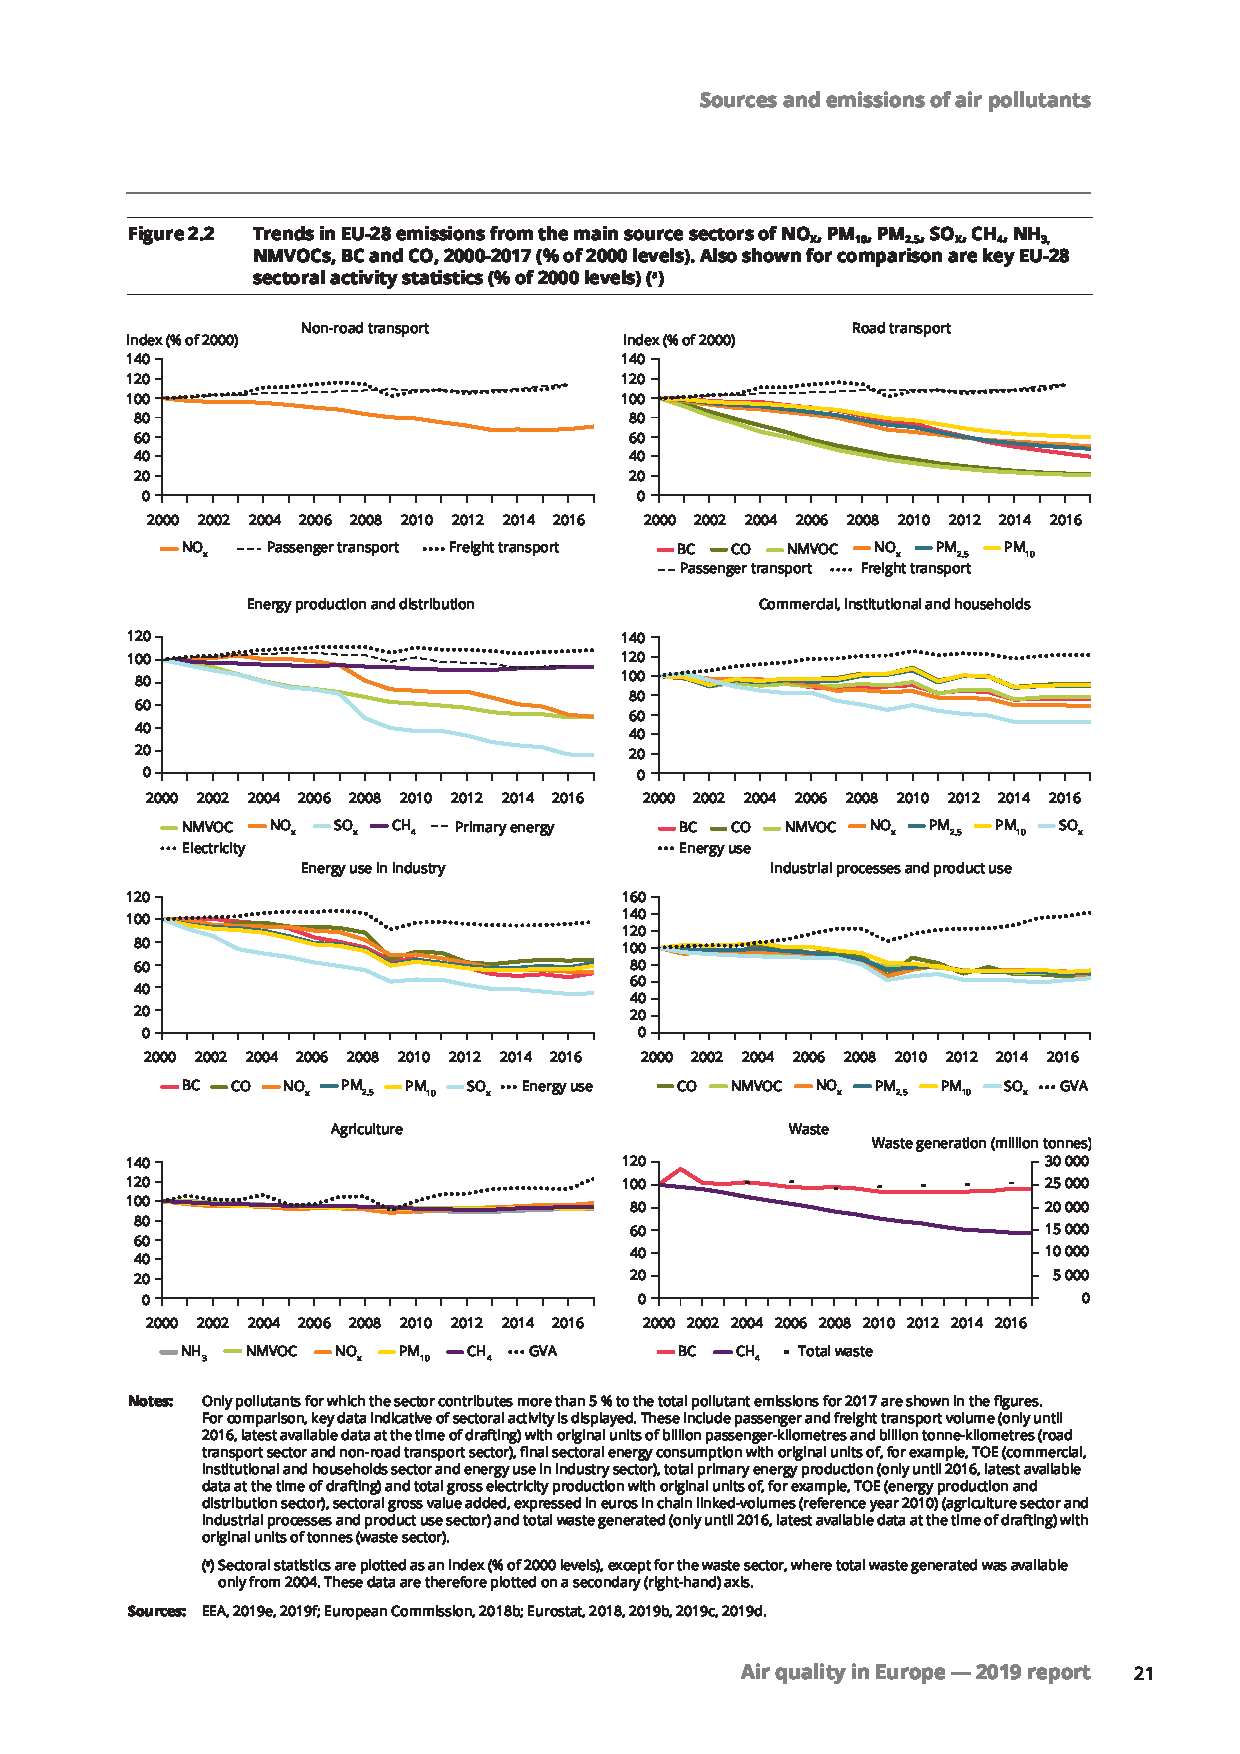
\includegraphics[clip,% left, bottom, right, top
        trim=0cm 6.5cm 0cm 5.3cm,%
        width=\textwidth]{img/pdf/european_emissions_by_sector.pdf}
    \caption{European emissions divided by activity sector. The global
    decreasing trend is confirmed, as industries all around are
    producing less and less \gls{AP} with the passing years~\cite{EEA2019}.}
    \label{fig:european_emissions_by_sector}
\end{figure}

\subsection{Detecting and Monitoring \acrlong{AP}}%
\label{sub:detecting_and_monitoring_ap}

There is no doubt that \gls{AP} is a global threat that affects
everyone, both in personal terms (through the degradation of their
health) and in societal terms, through the investments and limitations
that we as a whole have to commit to in order to prevent larger,
unmanageable problems. Reducing \gls{AP} is a priority and a requirement
for today's modern societies. This demands immediate and effective
actions, which in turn imply that we have a solid and profound
understanding of how pollutants are created, transported and transformed
in the atmosphere. The scale on which these interventions must be
conducted requires them to be made on a concerted and collaborative
manner, and always leveraged by technological
development~\cite{EEA2019}. Many of the air pollutants cannot be
detected solely by our senses, or even if they can is at already
dangerous concentrations. Technology is therefore a prerequisite to our
fighting the problem of \acrlong{AP}~\cite{Vallero2014}.

Pollution monitoring is itself based on the ability of a given
measurement method to determine concentrations for trace gases, aerosols
or radiation quantities. As with many other test techniques, in various
fields, pollution monitoring techniques have three very important
aspects to verify. The first of which is sensitivity, and also the most
demanding. Important trace gases in atmospheric chemistry have sometimes
vestigial concentrations, and the ability to correctly detect them is
many times a technical challenge. The second most important is
specificity, which is the ability of an atmospheric measurement to
measure each compound independently, without a component influencing
another component's measurement either positively or negatively.
Finally, any usable monitoring technique must be sufficiently precise as
to provide valid measurements.

\acrlong{AP} monitoring techniques and devices are too many to address
them all in this document. Besides, the physical principles involved are
completely different from one to another, making it very difficult to
make a broad generalization, other than the fact that they can be
divided into local and remote sensing devices. The gold standard for air
quality measurements remains those techniques in which a sample is
collected in the field and then taken to the laboratory to be analyzed
by very powerful analytical methods such as chromatography or mass
spectroscopy. While undoubtedly providing the most accurate
representation of the air composition at the time and place the sample
was collected, it is also true that this method's results are too slow
to use regularly in the field.

Another very important air quality monitoring method is the use of
electrochemical sensors. The first variants (wet cells) of this kind of
sensor became very popular in the field of industrial hygiene, where
they were applied in many portable flue gas analyzers. They were very
attractive to companies worldwide given their potential for very low
costs in comparison to optical or other more complex techniques. Apart
from the oxygen wet cell sensor, that has a slightly different
configuration, these electrochemical devices are comprised of three
electrodes - a sensing electrode, a counter electrode and a reference
electrode - separated by a thin layer of electrolyte. The gas that is
diffused to the surface of the electrode is either oxidized or reduced,
thus changing the systems electrical properties, in a way that is then
captured by an amplification circuit.

Wet cell electrochemical sensors were the precursors of the now more
common solid state sensors. These sensors are the ones that we see in
every subterranean parking lot, measuring several traffic related gases
such as \gls{co}, \gls{co2} or \gls{no2}. In general semiconductor gas
detectors are comprised of two modules: a receptor and a transducer (see
Figure~\ref{fig:semiconductor_sensor}). The receptor has in its
composition a material (or set of materials) that, in contact with the
target gas, induces a change in the systems inherent properties (work
function, dielectric constant, resistance, etc.) or emits heat or light.
The transducer is a device or circuit that converts the receptor's
changes into an electrical signal. There are 5 types of semiconductor
sensors, according to the material from which the transducer is made.
These types are enumerated in Table~\ref{tab:semiconductor_sensor}.

\begin{figure}[htpb]
    \centering
    \missingfigure{}
    \caption{Semiconductor electrochemical sensor basic structure. There
    are many examples of this type of sensors, but in general they
    follow this architecture.}
    \label{fig:semiconductor_sensor}
\end{figure}

\begin{table}[htpb]
    \centering
    \caption{Categorization of semiconductor gas sensors. The type of
    transducer and receptor dictates the type of the sensor.}
    \label{tab:semiconductor_sensor}
    \missingfigure{This is actually a table}
\end{table}

Optical (spectroscopic) systems are fundamentally different from the
other techniques that have already been presented. They can be used to
perform remote sensing measurements (as far as being used for
measurements aboard satellites). In the last few decades, these
techniques have gained a lot of ground in atmospheric research, due to
their high sensitivity and specificity and the universality of their
applicability. Spectroscopic methods are based on Lambert-Beer's law
(see Section~\ref{sec:doas} for a more thorough explanation), and make
use of the fact that the way in which gases interact with light is well
known and follows an exponential expression. There are many
spectroscopic techniques for measuring \gls{AP}. Selecting one requires
careful consideration of a number of factors like the target gases,
optical path arrangement, type of light source, etc.
Figure~\ref{fig:selecting_spectroscopic_method} provides several
examples of optical measurement methods, and how they can be divided.

\begin{figure}[htpb]
    \centering
    \missingfigure{}
    \caption{There are many spectroscopic techniques for atmospheric
    trace gas concentration measurement. Although several are depicted
    here, keep in mind that this is not an exhaustive list and is meant as
    an example repository.}
    \label{fig:selecting_spectroscopic_method}
\end{figure}

One of the most important atmospheric analysis methods, and especially
in what concerns this document, is \gls{DOAS}. While it is based on the
same mathematical formulation as the other spectroscopic methods, it is
also based on other factors, which shall be discussed in
Section~\ref{sec:doas}.

